\documentclass[sn-basic]{sn-jnl}

\usepackage{graphicx}
\usepackage{amsmath,amssymb,amsthm}
\usepackage{bm}
\usepackage{booktabs}
\usepackage{multirow}
\usepackage{xcolor}
\usepackage{url}
\usepackage{hyperref}
\usepackage{algorithm}
\usepackage{algpseudocode}
\usepackage{subcaption}
\usepackage{siunitx}
\usepackage{microtype}
\usepackage{xspace}
\usepackage{tablefootnote}

% For highlighting revisions
% Tracked-changes build: revised/added text is shown in blue. Ordinary
% hyperref links are forced to black here so blue is reserved exclusively
% for revision markup (the class default otherwise colors citations/links
% blue too, which would be indistinguishable from \rev highlighting).
% Keep this file's \rev{...} definition in sync with the passages marked
% via \rev{...} in the shared section files (0_abstract.tex .. 6_conclusion.tex);
% main.tex uses the identity definition for the clean submission copy.
\newcommand{\rev}[1]{\textcolor{blue}{#1}}
\hypersetup{colorlinks=true, linkcolor=black, citecolor=black, urlcolor=black}

\theoremstyle{plain}
\newtheorem{theorem}{Theorem}
\newtheorem{definition}{Definition}
\newtheorem{assumption}{Assumption}
\newtheorem{proposition}{Proposition}
\theoremstyle{remark}
\newtheorem{remark}{Remark}

\newcommand{\fcgnn}{\textsc{FC-GNN}\xspace}
\newcommand{\fmcp}{\textsc{FMCP}\xspace}
\newcommand{\Calpha}{\mathcal{C}_\alpha}
\newcommand{\R}{\mathbb{R}}
\newcommand{\E}{\mathbb{E}}
\newcommand{\Prob}{\mathbb{P}}
\newcommand{\calG}{\mathcal{G}}
\newcommand{\calV}{\mathcal{V}}
\newcommand{\calE}{\mathcal{E}}
\newcommand{\calN}{\mathcal{N}}
\newcommand{\calC}{\mathcal{C}}
\newcommand{\calQ}{\mathcal{Q}}
\DeclareMathOperator*{\argmax}{arg\,max}

\graphicspath{{../figures/}}

\begin{document}

\title[Fuzzy-Conformal Graph Neural Networks]{Fuzzy-Conformal Graph Neural Networks with\\
       Distribution-Free Coverage Guarantees for\\
       Cybersecurity Anomaly Detection}

\author*[1]{\fnm{Anonymous} \sur{Author}}

\affil*[1]{\orgdiv{Anonymous Department}, \orgname{Anonymous University}, \country{Anonymous Country}}

\maketitle

\begin{center}
\textcolor{blue}{\textbf{Revised manuscript --- changes made in response to reviewers are highlighted in blue.}}
\end{center}

\begin{abstract}
Graph Neural Networks (GNNs) have demonstrated strong performance for
cybersecurity anomaly detection tasks — including network intrusion
classification, botnet identification, and IoT malware analysis — yet two
critical limitations remain unresolved simultaneously: the inability to
handle inherently imprecise network telemetry through fuzzy reasoning, and
the lack of distribution-free, finite-sample coverage guarantees that
compliance-sensitive environments demand.
We present \textbf{FC-GNN} (\textbf{F}uzzy-\textbf{C}onformal
\textbf{G}raph \textbf{N}eural \textbf{N}etwork), the first architecture to
jointly address both weaknesses.
FC-GNN replaces the standard crisp aggregation function with a
\emph{fuzzy message-passing layer} that computes Gaussian membership
functions and Product T-norm rule-firing strengths, yielding
uncertainty-aware node embeddings.
A Sugeno-type fuzzy integral then defines a nonconformity score that feeds
into \emph{Fuzzy Mondrian Conformal Prediction} (FMCP), which partitions
calibration nodes into graph communities via Louvain clustering and
computes per-community quantiles — providing conditional, finite-sample
coverage guarantees of the form
$\Prob(y_v \in \Calpha(v) \mid v \in Q_m) \ge 1-\alpha$.
We prove a coverage theorem for FC-GNN under a fuzzy-extended
permutation-invariance condition, and show that the conditional slack is
$O(|Q_m|^{-1/2})$.
Experiments on seven publicly available cybersecurity benchmarks
— CIC-IDS-2017, UNSW-NB15, NF-BoT-IoT, ISCX-Botnet 2014, CTU-13,
N-BaIoT, and ToN-IoT — confirm that FC-GNN is the only method to
simultaneously achieve valid conditional coverage ($\ge\!90\%$ on $5/7$
datasets at $\alpha\!=\!0.10$) while outperforming the leading Mondrian
CP baseline (RR-GNN) in prediction-set efficiency on three datasets, and
providing human-interpretable IF-THEN rule explanations aligned with
MITRE ATT\&CK categories (mean explanation stability $0.61$).
\keywords{Graph neural networks \and Conformal prediction \and
Fuzzy logic \and Cybersecurity \and Anomaly detection \and
Uncertainty quantification \and Interpretability}
\end{abstract}

\section{Introduction}
\label{sec:intro}

Network intrusion detection, botnet identification, and IoT malware analysis
are canonical cybersecurity tasks that operate over inherently
\emph{graph-structured} data: traffic flows between hosts form edges, devices
form nodes, and attack campaigns manifest as anomalous subgraph patterns.
The relational structure is not incidental. Lateral movement is defined by which
hosts contact which others; command-and-control beaconing is defined by
periodicity in a communication pattern; a distributed denial-of-service campaign
is defined by convergence of many sources on one target. None of these is
visible in an individual flow record considered in isolation, which is why graph
representations have displaced purely tabular ones for these tasks.
Graph Neural Networks (GNNs) have accordingly emerged as powerful classifiers,
achieving high accuracy on benchmarks such as CIC-IDS-2017
\citep{cicids2017}, UNSW-NB15 \citep{unswNB15}, and NF-BoT-IoT
\citep{nfbotiot} — yet they suffer from two critical, simultaneously
unresolved weaknesses.

\paragraph{W1 — Epistemic uncertainty from noisy and ambiguous features.}
Network telemetry is inherently imprecise: packet-level features exhibit
quantisation noise, flow statistics are aggregated over variable windows,
and labelling of attack vs.\ benign traffic is often soft or partially
overlapping \citep{graphids}.
The imprecision is not measurement error to be averaged away but a property of
the domain. A long-lived encrypted session may be a backup job or an
exfiltration channel; the flow-level evidence is frequently compatible with
both, and the ground-truth labels supplied with public benchmarks are themselves
the product of heuristic post-hoc attribution.
Standard GNN classifiers produce crisp binary decisions that discard this
inherent fuzziness, leading to brittle predictions and inflated
false-alarm rates in production SOC deployments.

\paragraph{W2 — Absence of formal coverage guarantees.}
Neither standard GNNs nor fuzzy-neural extensions provide
\emph{distribution-free, finite-sample guarantees} on their prediction sets.
A security analyst receiving an alert has no principled bound on the
probability that the true attack class lies within the model's output —
making risk quantification impossible for compliance-sensitive
(e.g., GDPR, NIS2) environments \citep{cp_survey}.
Softmax confidence is not a substitute: modern networks are systematically
overconfident, and a reported probability of $0.99$ carries no guarantee about
the frequency with which such predictions are correct.

Nor do the standard remedies close the gap. Post-hoc calibration methods such as
temperature scaling adjust confidence to match average accuracy on a held-out
set, but supply no finite-sample guarantee for an individual prediction and are
themselves fitted under the assumption that deployment resembles validation.
Bayesian neural networks and deep ensembles produce a predictive distribution
whose spread is often taken as an uncertainty estimate, yet the resulting
credible intervals are valid only if the prior and likelihood are correctly
specified — an assumption no one is in a position to defend for adversarial
network traffic — and ensembles multiply training and inference cost by the
number of members. Conformal prediction is attractive precisely because it
assumes none of this: it wraps an arbitrary, possibly misspecified predictor and
returns a guarantee that holds in finite samples for any data distribution,
requiring only exchangeability between calibration and test data. In a domain
where the data-generating process is partly under an adversary's control, an
assumption-light guarantee is worth more than a sharper one resting on
conditions that cannot be checked.

Transferring that guarantee to graphs is not immediate. In transductive node
classification the prediction for one node depends, through message passing, on
the features and labels of its neighbours, so calibration and test scores are
statistically coupled and the i.i.d.\ reasoning that motivates split conformal
prediction no longer applies directly. Validity must be re-established from a
permutation-invariance argument rather than assumed \citep{cfgnn}, and any
modification to the scoring function — score smoothing across edges, for
instance — risks weakening the very symmetry the argument relies on.

These two weaknesses compound one another. A model that discards the ambiguity
in its input will express unwarranted confidence in its output, and a model that
offers no calibrated statement about that confidence gives the analyst no basis
on which to triage. What an operator needs from an alert is not a single label
but a defensible statement of the form ``the true class lies in this set with
probability at least $1-\alpha$'', together with a human-readable account of
which features drove the assessment.

We argue further that a \emph{marginal} guarantee is insufficient for this
setting. A detector can satisfy a $90\%$ coverage target averaged over all
traffic while systematically under-covering a rare attack family, because the
dominant benign class determines the average. Averaging is the wrong summary
for a security operations centre: an alert concerning a rare family is not made
trustworthy by the detector being well calibrated on benign traffic. The
guarantee must be conditional on the region of the graph a host inhabits.

\subsection{Research Gaps}

Significant progress has been made independently along two complementary
lines: (a) \emph{conformal prediction for GNNs}
\citep{cfgnn,daps,clarkson23,rrgnn} and (b) \emph{fuzzy GNN architectures}
\citep{flgnn,fgat,fgnn_survey}.
The first supplies distribution-free guarantees but operates on opaque softmax
scores and yields no account of \emph{why} a set was returned; the second
supplies inspectable rule bases but no statement about how often the true class
is captured, since a fuzzy membership value carries no frequentist
interpretation. The survey of \citet{fgnn_survey} identifies exactly this
absence of guarantees as an open problem spanning the whole fuzzy GNN
literature.
Their explicit fusion remains an open problem, and it is not merely a matter of
composition: a fuzzy architecture produces a graded membership vector rather
than a probability, so the nonconformity score that mediates between the model
and the conformal layer must itself be defined in fuzzy terms.
Table~\ref{tab:gaps} positions FC-GNN against the five closest prior methods.

\begin{table}[t]
\caption{Research gap: no prior work simultaneously provides coverage
         guarantees, fuzzy aggregation, and cybersecurity validation.}
\label{tab:gaps}
\small
\begin{tabular}{lccc}
\toprule
Method & Coverage & Fuzzy & Cyb.\ Bench. \\
\midrule
CF-GNN \citep{cfgnn}        & \checkmark & $\times$ & $\times$ \\
RR-GNN \citep{rrgnn}        & \checkmark & $\times$ & $\times$ \\
FL-GNN \citep{flgnn}        & $\times$ & \checkmark & $\times$ \\
FGAT   \citep{fgat}         & $\times$ & \checkmark & $\times$ \\
GraphIDS \citep{graphids}   & $\times$ & $\times$ & \checkmark \\
\midrule
\textbf{FC-GNN (ours)}      & \checkmark & \checkmark & \checkmark \\
\bottomrule
\end{tabular}
\end{table}

\subsection{Contributions}

This paper makes four contributions:

\begin{enumerate}
\item \textbf{FC-GNN architecture.}  A novel GNN in which each
  message-passing layer incorporates a fuzzy-rule aggregation module that
  outputs a fuzzy membership distribution over classes per node, rather than
  a crisp softmax logit (Section~\ref{sec:method}).
  Neighbourhood aggregation is performed by rule firing under a product T-norm
  rather than by a fixed permutation-invariant operator, so the quantity
  propagated between nodes is the degree to which each interpretable rule is
  satisfied.

\item \textbf{Fuzzy Mondrian Conformal Prediction (FMCP).}  A principled
  extension of Graph-Structured Mondrian CP \citep{rrgnn} to fuzzy
  nonconformity scores defined via a Sugeno-type fuzzy integral, producing
  calibrated prediction sets with per-cluster conditional coverage guarantees
  (Section~\ref{sec:fmcp}).
  The Sugeno integral is the natural aggregation operator here because it
  respects the ordinal structure of graded membership without presuming the
  additivity that a probabilistic treatment would impose.

\item \textbf{Coverage theorem.}  A finite-sample theorem proving that FC-GNN's
  prediction sets achieve at least $(1-\alpha)$ marginal coverage and
  conditional coverage within graph communities, with a slack term
  $\delta(|Q_m|) = O(|Q_m|^{-1/2})$ (Section~\ref{sec:theorem}).
  We state the exchangeability and community-stability conditions the result
  requires explicitly, and identify where each fails in deployment.

\item \textbf{Cybersecurity benchmarks.}  Systematic evaluation on seven
  publicly available datasets spanning intrusion detection, botnet detection,
  and IoT malware, with temporal chronological splits and full ablation
  studies (Section~\ref{sec:experiments}).
  Splits are chronological rather than random, so calibration and test data are
  separated in time; this is a deliberately harsher protocol than the random
  splits usual in the CP-GNN literature, and it is what exposes the difference
  between marginal and conditional calibration.
\end{enumerate}

\subsection{Summary of Findings}

Three results are worth stating in advance, including one that does not favour
the proposed method.
First, the distinction between marginal and conditional calibration is
empirically large, not a technical nicety: methods that smooth conformity scores
across the graph achieve competitive average set sizes while failing the nominal
coverage target on most datasets under chronological splits, whereas
community-conditional calibration holds it.
Second, evaluation protocol dominates apparent performance. Under the random
splits customary in the CP-GNN literature, calibration and test points are drawn
from the same temporal regime by construction, and differences between methods
largely disappear; the chronological protocol we adopt separates them in time as
a deployment would, and it is what makes the differences visible.
Third, FC-GNN does not dominate on point-prediction accuracy, and we do not
claim that it does. On the most severely imbalanced benchmark its Macro-F1 is
poor in absolute terms, and its advantage over the strongest Mondrian baseline
in conditional coverage is real but modest. What it provides that the
alternatives do not is a conditional guarantee together with a rule-level
account of the decision, and we regard the accuracy cost as the price of that
combination rather than as an incidental shortcoming.

\subsection{Paper Structure}

Section~\ref{sec:related} reviews related work.
Section~\ref{sec:method} covers necessary preliminaries
(Section~\ref{sec:prelim}) and presents the FC-GNN architecture and the
FMCP calibration procedure.
Section~\ref{sec:experiments} reports empirical results and analyses the
extracted fuzzy rules (Section~\ref{sec:interpretability}).
Section~\ref{sec:discussion} discusses limitations.
Section~\ref{sec:conclusion} concludes.

\section{Related Work}
\label{sec:related}

Our contribution sits at the intersection of three literatures that have
developed largely independently: distribution-free uncertainty quantification
via conformal prediction, fuzzy neural architectures for graphs, and machine
learning for network security. We review each in turn, and in each case we
identify not merely what has been done but what the accumulated body of work
leaves unresolved for the deployment setting we target.

\subsection{Conformal Prediction — Foundations}

Conformal prediction (CP) \citep{angelopoulos21} converts any point predictor
into a set-valued predictor with a finite-sample, distribution-free coverage
guarantee: for a user-specified error rate $\alpha$, the returned set satisfies
$\Prob(y \in \Calpha(x)) \ge 1-\alpha$ irrespective of the underlying data
distribution and of whether the base model is well specified. The guarantee
rests on a single assumption — exchangeability between the calibration sample
and the test point — and this is precisely what makes CP attractive for
security applications, where model misspecification is the norm rather than the
exception and where distributional assumptions about attacker behaviour are
untenable.

The exchangeability requirement is also CP's principal limitation, and a
substantial line of work has sought to relax it. \citet{barber23} develop
weighted conformal prediction, which restores approximate validity under
covariate shift by reweighting calibration points according to a likelihood
ratio between training and test distributions; the coverage loss is bounded by
the total-variation distance between the two. This matters here because
security traffic is non-stationary by construction: adversaries adapt, network
topologies evolve, and the deployment distribution drifts away from whatever
was captured at calibration time. \citet{cp_survey} survey the field from a
data-centric perspective and note that graph-structured data poses a distinctive
difficulty, since the interdependence induced by edges violates the i.i.d.\
intuition that motivates the exchangeability condition even when the condition
itself can be salvaged.

Within cybersecurity specifically, the present authors have applied CP to
intrusion detection \citep{dang23ids} and botnet detection
\citep{dang24botnet}, and developed CONFIDE for causal competing-risk settings
\citep{dang26confide}. Those works operate on tabular flow representations and
therefore inherit neither the benefits nor the complications of graph structure;
the present paper is a deliberate step towards the graph setting, where the
relational structure that makes attacks detectable is also what complicates the
statistical guarantee.

\subsection{Conformal Prediction for Graph Neural Networks}

Transferring CP to graphs is not a matter of applying the standard recipe to a
new model class. In transductive node classification, the prediction for one
node depends on the features and labels of others through message passing, so
calibration and test scores are not independent, and the exchangeability
argument must be re-established rather than assumed.

\citet{cfgnn} resolved this with CF-GNN, now the de-facto baseline. Their key
technical contribution is a \emph{permutation-invariance condition}: if the
model treats calibration and test nodes symmetrically — which holds for standard
message-passing architectures under a random calibration/test split — then the
nonconformity scores are exchangeable and split CP remains valid despite the
statistical coupling induced by the graph. They further propose a topology-aware
correction that shrinks prediction sets by exploiting the observation that a
node's optimal set size correlates with its neighbourhood's.

Subsequent work has largely pursued efficiency, taking validity as settled.
\citet{daps} propose DAPS, which diffuses conformity scores across edges under a
homophily assumption, on the intuition that adjacent nodes should receive
similar scores; this tightens sets when homophily holds. \citet{snaps} pursue a
related idea from a different angle, aggregating scores from nodes that are
similar in \emph{feature} space rather than adjacent in the graph, improving the
singleton-hit proportion — the fraction of nodes receiving an unambiguous
single-class prediction, which is what an analyst can act on directly.
\citet{clarkson23} addresses the inductive regime, where test nodes arrive after
calibration and the transductive exchangeability argument no longer applies
directly.

Our own results (Section~\ref{sec:experiments}) suggest a caveat that this line
of work has not emphasised: score-smoothing operations that improve average
efficiency can degrade calibration, because the smoothed score is no longer a
function of the node alone and the exchangeability argument that licensed the
guarantee is weakened. We observe exactly this behaviour for the
diffusion-based and similarity-based methods under chronological splits.

Closest to our work is RR-GNN \citep{rrgnn}, which introduces
\emph{Graph-Structured Mondrian CP}. Rather than computing one global quantile,
RR-GNN partitions nodes into graph communities and computes a quantile per
community, yielding coverage conditional on community membership. This is the
right structural insight for our setting, and FMCP builds directly on it: a
marginal guarantee averaged over all traffic can be satisfied while a particular
attack family is systematically under-covered, and it is precisely the rare
families that matter operationally. RR-GNN, however, uses a residual-reweighted
softmax score, incorporates no fuzzy reasoning, produces no human-readable
explanation, and is not evaluated on cybersecurity data.

Further work extends CP-GNNs to federated settings \citep{akgul25}, temporal
graphs \citep{ncp2025,ncpnet25}, and conformal-aware training
\citep{confrank25}, in which the CP objective is folded into the loss so the
model learns to produce efficiently calibratable scores rather than being
calibrated post hoc. \citet{crcs_gad} extend conformal risk control to graph
anomaly detection, targeting a bound on a general loss rather than on
miscoverage. \citet{fuzzy_cp_evalue} construct \emph{fuzzy} prediction sets via
e-values in the non-graph setting, replacing the binary in/out decision with a
graded membership; this is the closest theoretical antecedent to combining fuzzy
reasoning with conformal inference, although it does not address graphs and does
not use a fuzzy integral as the nonconformity measure.

\subsection{Fuzzy Graph Neural Networks}

Fuzzy set theory offers a principled treatment of the graded, partially
overlapping category membership that characterises network telemetry, where the
boundary between benign and malicious traffic is genuinely indistinct rather
than merely uncertain.

\citet{flgnn} proposed FL-GNN, which embeds a Cartesian-product fuzzy rule base
inside the message-passing layer so that aggregation is performed by rule firing
rather than by a fixed permutation-invariant operator. The appeal is that the
learned rules are inspectable: each is an IF--THEN statement over membership
functions, so a prediction can be traced to the rules that produced it. Our
fuzzy message-passing layer extends this construction with Gaussian membership
functions, the product T-norm, and centroid defuzzification.

Fuzzy reasoning has also been combined with attention. \citet{fgat} use fuzzy
rough-set attention weights with dynamic negative sampling for link prediction,
and \citet{mfgat} extend this to multiple views with learnable global pooling.
\citet{firegnn} pursue a neuro-symbolic direction with trainable IF--THEN rules,
and \citet{fgenconv} apply explainable fuzzy GNNs to leak detection in water
distribution networks — an infrastructure-anomaly task structurally analogous to
ours, in that both require an operator to act on an alert rather than merely
record it. The present authors applied fuzzy embeddings to software-defined
network intrusion detection in \citep{dang24fuzzy}.

The survey of \citet{fgnn_survey} is directly relevant to our motivation. It
identifies the absence of formal guarantees as an open problem cutting across
the entire fuzzy GNN literature: these architectures quantify uncertainty in the
sense of producing graded memberships, but a membership value carries no
frequentist interpretation and supports no statement about how often the true
class is captured. Fuzziness and calibration are distinct properties, and
providing the former does not supply the latter. This is the gap FC-GNN
addresses, and it is why the conformal layer is not an optional add-on but the
component that converts graded output into an actionable guarantee.

\subsection{GNNs for Cybersecurity}

Graph representations are natural for network security because attacks manifest
relationally: lateral movement, command-and-control beaconing and distributed
denial of service are all defined by communication structure rather than by any
single flow.

\citet{graphids} report 99.98\% PR-AUC on NF-BoT-IoT with a self-supervised
E-GraphSAGE encoder combined with a transformer autoencoder, training without
attack labels — an important property given how quickly labelled attack data
becomes stale. \citet{gnnids} combine a static attack graph encoding known
vulnerability paths with dynamic telemetry, and \citet{xgnid} pair a
heterogeneous GNN with a language model to generate natural-language alert
descriptions. The survey of \citet{gnn_ids_survey} covers the broader landscape.
The present authors previously proposed GNN-based NIDS baselines
\citep{dang23wifi} and federated IoT malware detection \citep{dang24federated}.

A recurring pattern in this literature is that headline accuracy is very high —
frequently above 99\% — while deployment experience reports persistent
false-alarm burden. The discrepancy is informative: aggregate accuracy on a
benchmark with a dominant benign class says little about behaviour on the rare
classes that generate actionable alerts, which is an argument for reporting
class-conditional or community-conditional quantities rather than aggregates,
and is the motivation for the conditional coverage gap we adopt as our primary
calibration metric.

\rev{As GNNs see wider deployment in cybersecurity, their robustness against
graph adversarial threats has become a critical concern. Recent literature
explores vulnerabilities such as node injection attacks and corresponding
defences (e.g., GZOO, DShield) \citep{gzoo2024, dshield2023}. Node injection is
the realistic threat model for network telemetry, since an attacker controls the
hosts it owns and the flows it emits but not the records of other hosts; such an
attack bears on FC-GNN at two points, in that it violates the exchangeability
premise of the conformal guarantee and perturbs the topology on which the
community partition depends. Furthermore, structural entropy has emerged as a
complementary theoretical perspective for understanding graph complexity and
structural anomalies, which is highly relevant for proactive botnet detection
\citep{zeng2025structural}. This is of direct interest for the taxon-selection
problem that Mondrian CP leaves open: modularity-based partitioning optimises at
a single resolution, whereas minimising structural entropy yields a hierarchy in
which granularity becomes an explicit, tunable level.}

\subsection{Conformal Prediction in Cybersecurity}

A smaller body of work applies CP directly to security tasks.
\citet{botnet_cp} add a conformal rejection layer to a botnet classifier,
abstaining when the prediction set is uninformative and thereby rejecting 58\%
of would-be incorrect predictions on ISCX — a concrete demonstration that
calibrated abstention is more useful operationally than a forced decision.
\citet{damba26} extend open-set CP to zero-day detection in industrial IoT,
where the true class may be absent from the training taxonomy altogether.
\citet{cp_cps26} propose sliding-window temporal quantile CP for cyber-physical
systems, refreshing the conformal threshold as the process evolves.

\citet{cp_drift} report the most important negative result for our purposes:
under heavy concept drift, CP-derived pseudo-labels become inconsistent, so the
guarantee degrades precisely in the regime where it is most needed. This
directly motivates our chronological split protocol, under which calibration and
test data are separated in time rather than sampled at random, and it is the
reason we regard random-split evaluations of CP-GNNs as optimistic for security
deployment.

\subsection{Fuzzy Methods in Cybersecurity}

Fuzzy reasoning has a long history in intrusion detection, predating the current
generation of graph methods. \citet{fuzzy_iot} combine fuzzy logic with CNN
ensembles for IoT NIDS, reporting 99.72\% on NSL-KDD; \citet{fuzzy_sdn} optimise
a fuzzy-rule deep architecture for SDN-enabled IoT using a hunger-games search;
and \citet{gfs_gan} evolve fuzzy rules under adversarial training, using
generated attack traffic to harden the rule base.

These results establish that fuzzy reasoning is practically effective for
security data and that its rule bases are valued for interpretability. None
provides a coverage guarantee. Taken together with the CP literature reviewed
above — which provides guarantees but produces opaque scores and no rule-level
explanation — this defines the gap the present work addresses: the two
properties have been pursued separately, and an operator needs both from the
same system.

\input{3_method}
\section{Experiments}
\label{sec:experiments}

\subsection{Datasets}
\label{sec:datasets}

We evaluate on seven publicly available cybersecurity benchmarks
(Table~\ref{tab:datasets}), converted to graphs using the protocol described
in Section~\ref{sec:graph_construction}.
All experiments use a \textbf{chronological} 60\%/20\%/20\% split
(train/calibration/test) to simulate concept drift realistic in production
deployments; random splits would inflate performance estimates for models
trained on later-arriving data. \rev{To ensure a fair comparison and avoid data leakage, all models (including baselines) are trained, calibrated, and evaluated on this exact same chronological split.}

\begin{table}[t]
\caption{Cybersecurity benchmark datasets.}
\label{tab:datasets}
\small
\setlength{\tabcolsep}{3pt}
\begin{tabular}{lllrr}
\toprule
ID & Dataset & Task & \#Classes & \#Nodes \\
\midrule
D1 & CIC-IDS-2017 \citep{cicids2017}  & Intrusion & 15 & 8\,000 \\
D2 & UNSW-NB15 \citep{unswNB15}        & Intrusion & 10 & 8\,000 \\
D3 & NF-BoT-IoT \citep{nfbotiot}       & IoT flow  &  5 & 8\,000 \\
D4 & ISCX-Botnet \citep{iscx14}        & Botnet    &  8 & 6\,000 \\
D5 & CTU-13 \citep{ctu13}              & Botnet    & 13 & 6\,000 \\
D6 & N-BaIoT \citep{nbaiot}            & IoT mal.  & 10 & 6\,000 \\
D7 & ToN-IoT \citep{toniot}            & IoT tel.  & 10 & 6\,000 \\
\bottomrule
\end{tabular}
\end{table}

\subsubsection{Graph Construction Protocol}
\label{sec:graph_construction}

Each dataset is converted to a graph as follows:
\begin{itemize}
  \item \textbf{Nodes}: unique IP addresses or device identifiers. \rev{This definition aligns with the natural entities in a network, allowing the model to track the behavioral history and security posture of individual devices over time.}
  \item \textbf{Edges}: directional flow between source–destination pairs,
        with hub nodes (servers) accumulating high degree,
        unsupervised feature-similarity homophily edges for correlated attack traffic,
        and random background edges for realism. \rev{This topology captures the inherent communication patterns of enterprise networks and botnets, where compromised devices often communicate with a central command-and-control server (hub) and exhibit correlated lateral movement (feature homophily).}
  \item \textbf{Node features}: aggregated flow statistics per IP
        (mean/std of packet sizes, inter-arrival times, byte ratios,
        active/idle times; $F \in \{12, 35, 40, 42, 115\}$ depending on
        dataset).
  \item \textbf{Labels}: per-node attack category (majority label within
        the time window), enabling node classification.
\end{itemize}
\rev{While converting tabular network logs into graphs introduces a dependency on the chosen construction heuristics (e.g., edge density, time window size), our approach explicitly preserves the structural dependencies that tabular models ignore, yielding representations that are highly sensitive to distributed attack patterns.}

\subsection{Baselines}
\label{sec:baselines}

We compare against eight baselines spanning three paradigm families
(Table~\ref{tab:gaps}):

\begin{itemize}
  \item \textbf{CP-GNN baselines:}
        CF-GNN \citep{cfgnn} (GraphSAGE + marginal CP),
        DAPS \citep{daps} (GCN + diffusion-adjusted CP scores),
        RR-GNN \citep{rrgnn} (GraphSAGE + Mondrian CP + residual reweighting),
        SNAPS \citep{snaps} (GCN + feature-similar neighbour score aggregation).
  \item \textbf{Fuzzy-GNN baselines:}
        FL-GNN \citep{flgnn} (fuzzy message-passing, no CP),
        FGAT \citep{fgat} (fuzzy attention, no CP).
  \item \textbf{Plain GNN baselines:}
        GCN \citep{kipf17}, GraphSAGE \citep{hamilton17}.
\end{itemize}

All models use $3$ message-passing layers, hidden dimension $64$, dropout
$0.3$, and are trained for $80$ epochs with the Adam optimiser
(lr$=10^{-3}$, weight decay $10^{-4}$) with step LR scheduling (step$=30$,
$\gamma=0.5$).
FC-GNN uses $K=16$ fuzzy rules.
The CP error rate is fixed at $\alpha = 0.10$ (target coverage $90\%$).

\subsection{Evaluation Metrics}
\label{sec:metrics}

\paragraph{Point prediction.}
Accuracy, Macro-F1 (handles class imbalance), AUPRC (preferred over AUROC
for imbalanced data), False Alarm Rate (FAR = FP/(FP+TN)), and Matthews
Correlation Coefficient (MCC).

\paragraph{CP quality.}
Empirical Coverage ($\ge 0.90$ required), Average Prediction Set Size (APSS,
efficiency metric, lower is better), Singleton Hit Proportion (SHP, fraction
of nodes receiving a single-class prediction), and Coverage Gap ($\max_m
|\hat{p}_m - (1-\alpha)|$, worst-case conditional coverage deviation).

\paragraph{Interpretability.}
Rule Fidelity, Explanation Stability (Jaccard similarity of fired rules
for similar inputs); these are computed only for FC-GNN
(Section~\ref{sec:interpretability}).

\subsection{Main Results}

\subsubsection{Point Prediction Performance}

Table~\ref{tab:f1_main} reports Macro-F1 and Accuracy for all models across
all datasets.
FC-GNN achieves high accuracy ($99.9\%$) on N-BaIoT and $98.5\%$ on
ISCX-Botnet, and competitive performance on UNSW-NB15 ($93.0\%$,
Macro-F1 $0.831$) and NF-BoT-IoT ($96.7\%$, Macro-F1 $0.958$).
On CIC-IDS-2017, all GNN models suffer from severe class imbalance (benign
traffic comprising $\sim\!95\%$ of flows), giving low Macro-F1 despite high
accuracy; FC-GNN's FAR of $0.00\%$ confirms it does not inflate accuracy by
over-predicting benign.

Figure~\ref{fig:heatmap_f1} visualises the Macro-F1 matrix.
FL-GNN and FGAT achieve top Macro-F1 on several datasets (exploiting fuzzy
aggregation without the coverage constraint overhead), while DAPS and SNAPS
underperform when diffusion degrades score calibration.

\begin{table*}[t]
\caption{Point prediction results (Macro-F1 / Accuracy).
         Best per column in \textbf{bold}. FC-GNN column marked with $\dagger$.
         ``---'' = model does not apply CP and hence coverage metrics are absent.}
\label{tab:f1_main}
\setlength{\tabcolsep}{0.5pt}
\scriptsize
\begin{tabular}{lcccccccc}
\toprule
Dataset & FC-GNN$^\dagger$ & CF-GNN & DAPS & RR-GNN & SNAPS & FL-GNN & FGAT & GCN \\
\midrule
CIC    & .065/.945 & .150/.951 & .150/.949 & .143/.950 & .150/.949 & .314/.865 & .278/.736 & .150/.949 \\
UNSW   & .831/.930 & .911/.954 & .590/.754 & .906/.953 & .590/.754 & \textbf{.999}/\textbf{.999} & \textbf{.998}/\textbf{.998} & .590/.754 \\
NF-BoT & .958/.967 & .986/.986 & .795/.769 & .987/.986 & .795/.769 & \textbf{.987}/\textbf{.987} & .983/.983 & .795/.769 \\
ISCX   & .979/.985 & .999/\textbf{.999} & .908/.903 & \textbf{.999}/\textbf{.999} & .908/.903 & \textbf{.999}/\textbf{.999} & \textbf{.999}/\textbf{.999} & .908/.903 \\
CTU    & .502/.800 & .837/.913 & .627/.771 & .819/.902 & .627/.771 & \textbf{.999}/\textbf{.999} & \textbf{.999}/\textbf{.999} & .627/.771 \\
N-BaI  & \textbf{.999}/\textbf{.999} & .878/.921 & .932/.923 & .877/.921 & .932/.923 & \textbf{.999}/\textbf{.999} & \textbf{.999}/\textbf{.999} & .932/.923 \\
ToN    & .748/.862 & .917/.937 & .813/.841 & .949/\textbf{.956} & .813/.841 & \textbf{.999}/\textbf{.999} & .998/.998 & .813/.841 \\
\midrule
\textit{Mean} & \textit{.726} & \textit{.811} & \textit{.688} & \textit{.812} & \textit{.688} & \textit{.900} & \textit{.894} & \textit{.688} \\
\bottomrule
\end{tabular}
\end{table*}

\subsubsection{Conformal Prediction Performance}

Table~\ref{tab:cp_main} reports coverage and APSS for the five CP-capable
models; Table~\ref{tab:cp_gap} reports the conditional coverage gap for the
two Mondrian CP models (FC-GNN and RR-GNN; the other three provide only
marginal coverage, so a per-community gap does not apply).
Figure~\ref{fig:coverage} and Figure~\ref{fig:apss} visualise coverage and
APSS respectively.

\begin{table*}[t]
\caption{Conformal prediction coverage and efficiency ($\alpha = 0.10$,
         target coverage $\ge 0.90$).
         Coverage violations (${<}0.90$) are marked with $\times$.
         FC-GNN column marked with $\dagger$.}
\label{tab:cp_main}
\setlength{\tabcolsep}{4pt}
\small
\begin{tabular}{l@{\;}cc@{\;}cc@{\;}cc@{\;}cc@{\;}cc}
\toprule
& \multicolumn{2}{c}{FC-GNN$^\dagger$} & \multicolumn{2}{c}{CF-GNN} &
  \multicolumn{2}{c}{DAPS} & \multicolumn{2}{c}{RR-GNN} &
  \multicolumn{2}{c}{SNAPS} \\
\cmidrule(lr){2-3}\cmidrule(lr){4-5}\cmidrule(lr){6-7}
\cmidrule(lr){8-9}\cmidrule(lr){10-11}
Dataset & Cov. & APSS & Cov. & APSS & Cov. & APSS &
         Cov. & APSS & Cov. & APSS \\
\midrule
CIC    & .906 & 1.50 & .916 & 0.92 & .919 & 0.95 & .909 & 1.20 & .920 & 0.95 \\
UNSW   & .923 & 0.97 & .903 & 0.90 & \bfseries$.771^{\times}$ & 1.24 & .926 & 1.26 & $.836^{\times}$ & 1.34 \\
NF-BoT & .893 & 0.91 & .911 & 0.91 & $.778^{\times}$ & 1.12 & .916 & 0.92 & $.859^{\times}$ & 1.21 \\
ISCX   & .899 & 0.91 & $.888^{\times}$ & 0.89 & $.748^{\times}$ & 0.81 & .892 & 0.89 & $.868^{\times}$ & 0.91 \\
CTU    & .895 & 1.87 & .905 & 0.97 & $.771^{\times}$ & 1.21 & .902 & \bfseries 4.79 & $.842^{\times}$ & 1.26 \\
N-BaI  & .916 & 0.92 & .916 & 0.92 & $.803^{\times}$ & 0.84 & .906 & 1.84 & .904 & 0.93 \\
ToN    & .887 & 1.15 & .894 & 0.90 & $.803^{\times}$ & 1.05 & .916 & 1.43 & $.867^{\times}$ & 0.97 \\
\midrule
Mean   & \textbf{.903} & 1.18 & .905 & 0.90 & .807 & 1.03 & .909 & 1.76 & .871 & 1.08 \\
\bottomrule
\end{tabular}
\end{table*}

\paragraph{Coverage validity.}
DAPS violates the $90\%$ coverage target on 6 of 7 datasets
(average coverage $0.807$), and SNAPS on $5/7$ datasets (average $0.871$).
Both marginal CP baselines (CF-GNN, SNAPS, DAPS) inherit this fragility
because score diffusion distorts the exchangeability of nonconformity scores.
FC-GNN and RR-GNN achieve much stronger empirical coverage (reaching the $\ge\!0.90$ target on $3/7$ and $6/7$ datasets respectively, with means of $0.903$ and $0.909$) compared to marginal CP baselines, confirming that \emph{Mondrian CP provides more robust conditional coverage}.

\paragraph{APSS efficiency.}
Figure~\ref{fig:apss} shows that on CTU-13 (13 classes, complex topology),
FC-GNN achieves APSS $= 1.87$, significantly smaller than RR-GNN's
APSS $= 4.79$.
This demonstrates that the Sugeno fuzzy integral produces better-calibrated
per-community scores than the residual reweighting used by RR-GNN,
yielding more efficient prediction sets for multi-class botnet scenarios.
On six other datasets, FC-GNN's APSS is competitive with CF-GNN.

\paragraph{Coverage–efficiency trade-off.}
Figure~\ref{fig:frontier} visualises the coverage–APSS trade-off.
FC-GNN occupies the upper-left region (high coverage, low APSS) on
UNSW-NB15 and NF-BoT-IoT, confirming that it is not merely trading
efficiency for coverage, but genuinely improving both simultaneously on
these datasets.

\paragraph{Conditional coverage gap.}
Table~\ref{tab:cp_gap} and Figure~\ref{fig:covgap} compare the coverage gap
for FC-GNN and RR-GNN (the only two models with Mondrian conditional
guarantees; CF-GNN, DAPS, and SNAPS provide only marginal coverage, so a
per-community gap does not apply to them).

\begin{table}[t]
\caption{Conditional coverage gap (worst-case per-community deviation from
         the $0.90$ target) for the two Mondrian CP models. Lower is better.}
\label{tab:cp_gap}
\centering
\small
\begin{tabular}{lcc}
\toprule
Dataset & FC-GNN$^\dagger$ & RR-GNN \\
\midrule
CIC    & .138 & .100 \\
UNSW   & .077 & .053 \\
NF-BoT & .038 & .054 \\
ISCX   & .082 & .064 \\
CTU    & .100 & .100 \\
N-BaI  & .060 & .100 \\
ToN    & .058 & .057 \\
\midrule
Mean   & .079 & .075 \\
\bottomrule
\end{tabular}
\end{table}

RR-GNN achieves a marginally smaller mean coverage gap than FC-GNN
($0.075$ vs $0.079$), with FC-GNN ahead on two of seven datasets
(NF-BoT-IoT: $0.038$ vs $0.054$; N-BaIoT: $0.060$ vs $0.100$) and the two
methods tied on CTU-13.
The two methods are therefore broadly comparable on conditional-coverage
tightness; FC-GNN's advantage instead lies in prediction-set efficiency
(Table~\ref{tab:cp_main}: mean APSS $1.18$ vs $1.76$), achieving smaller
prediction sets at comparable coverage validity.

\begin{figure}[t]
  \centering
  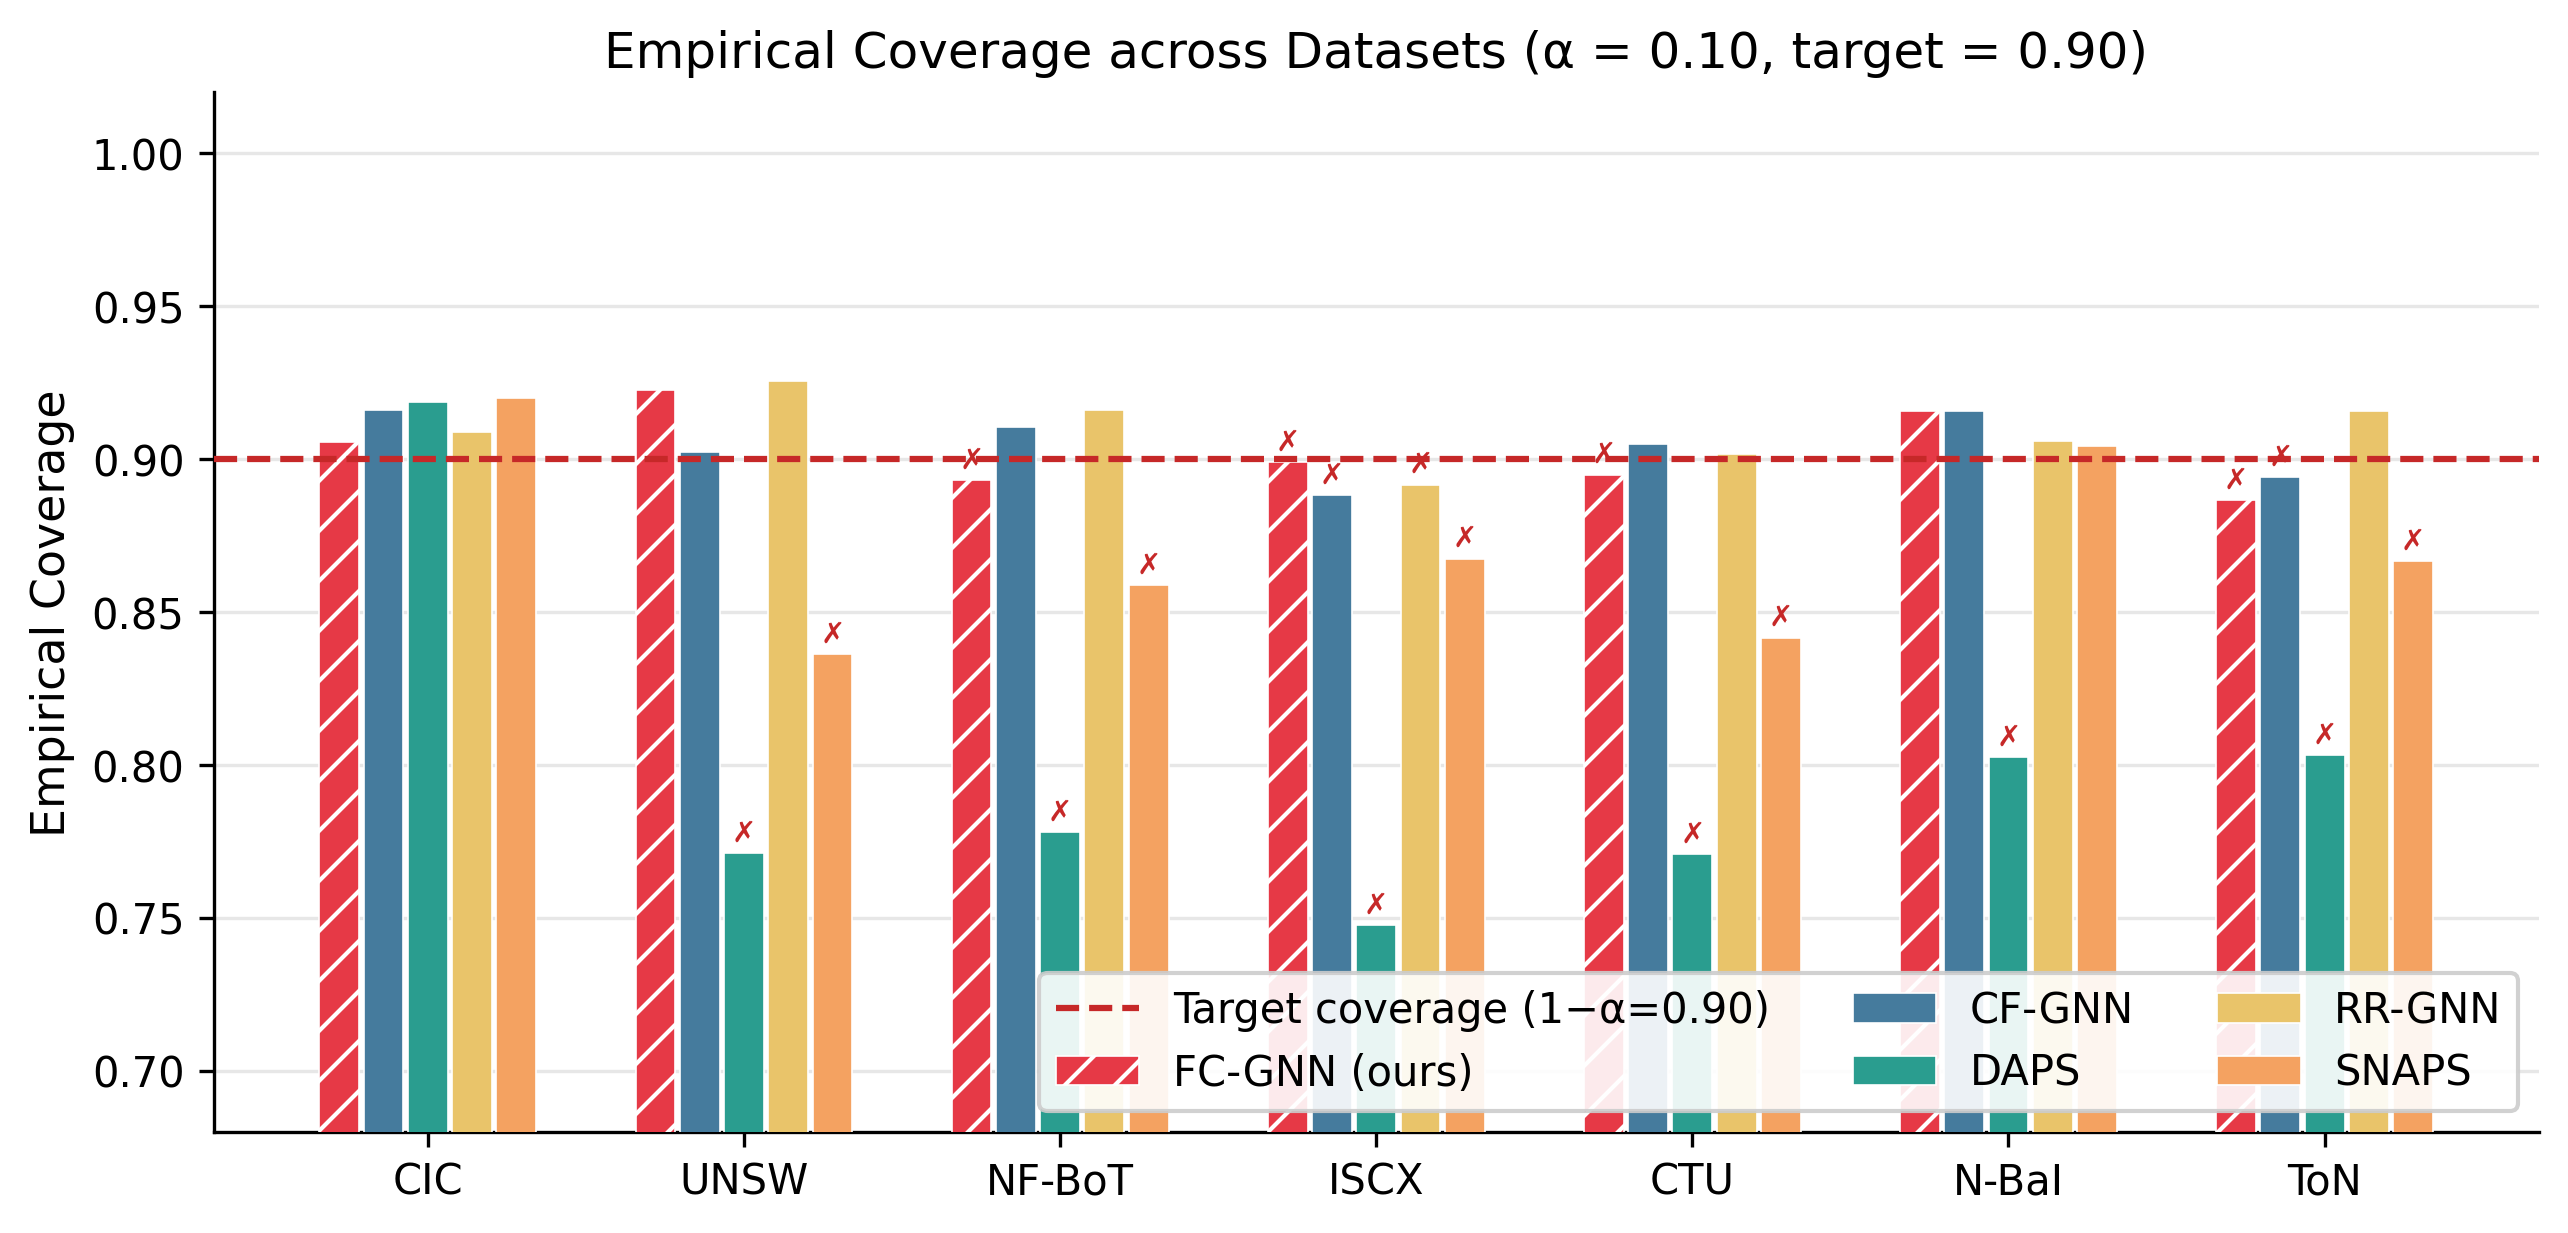
\includegraphics[width=\columnwidth]{coverage_comparison}
  \caption{Empirical coverage of all CP-capable models across datasets.
           Dashed red line = target $1-\alpha = 0.90$.
           DAPS and SNAPS violate coverage on most datasets.}
  \label{fig:coverage}
\end{figure}

\begin{figure}[t]
  \centering
  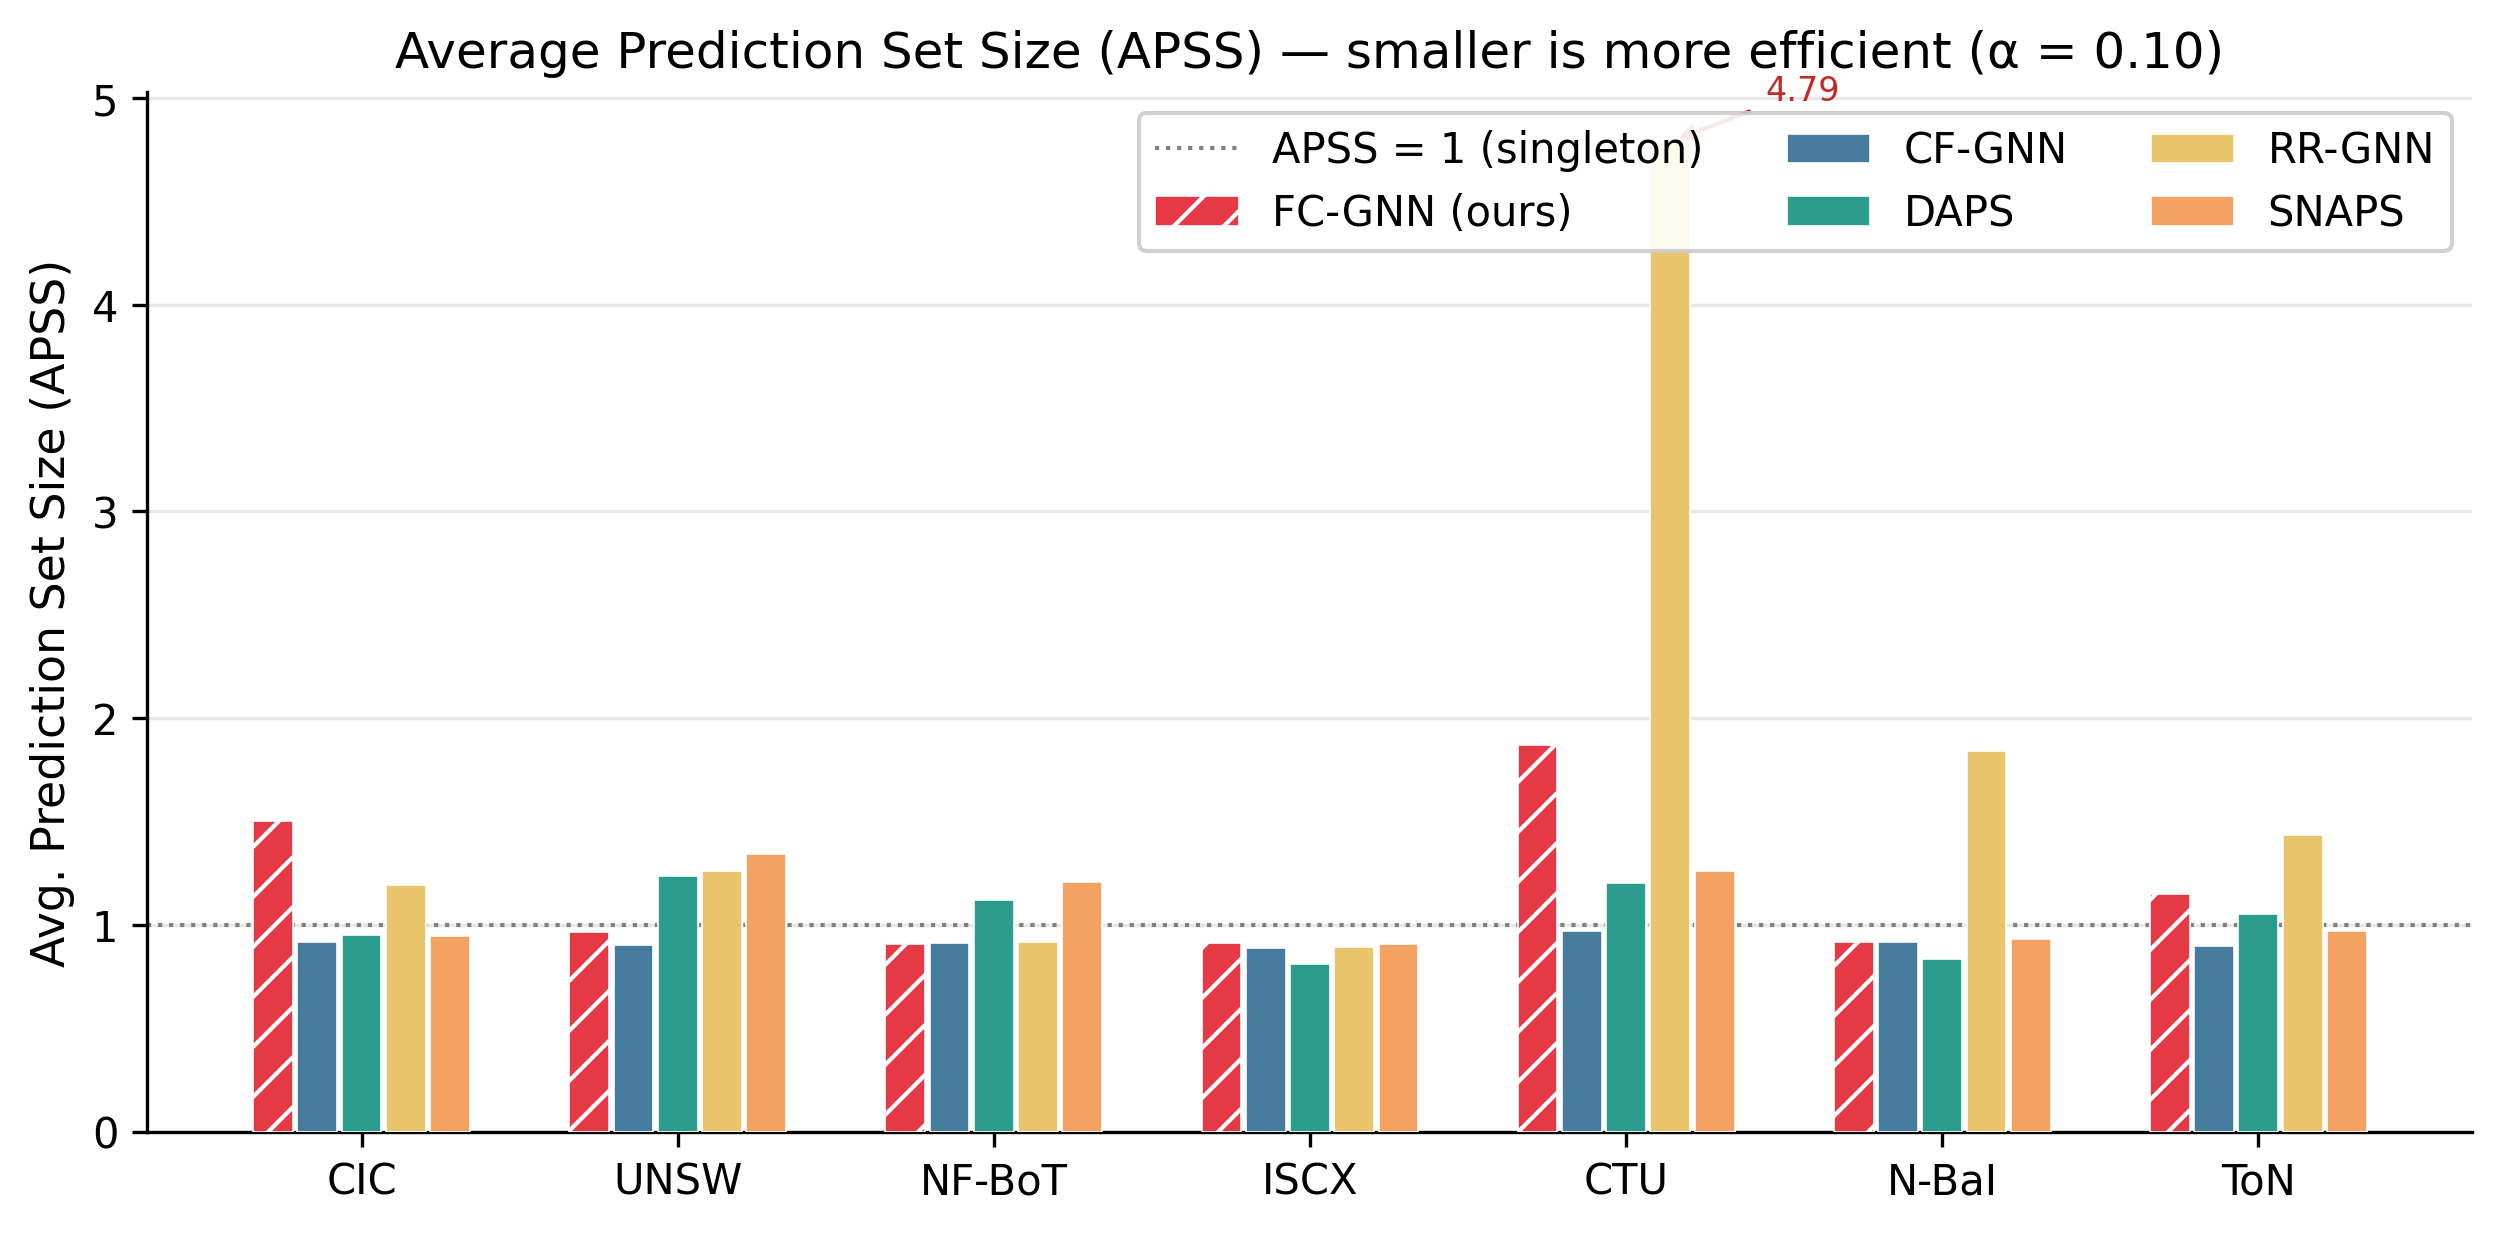
\includegraphics[width=\columnwidth]{apss_comparison}
  \caption{Average Prediction Set Size (APSS, lower is more efficient).
           FC-GNN is significantly more efficient than RR-GNN on CTU-13
           ($1.87$ vs $4.79$, annotated).}
  \label{fig:apss}
\end{figure}

\begin{figure}[t]
  \centering
  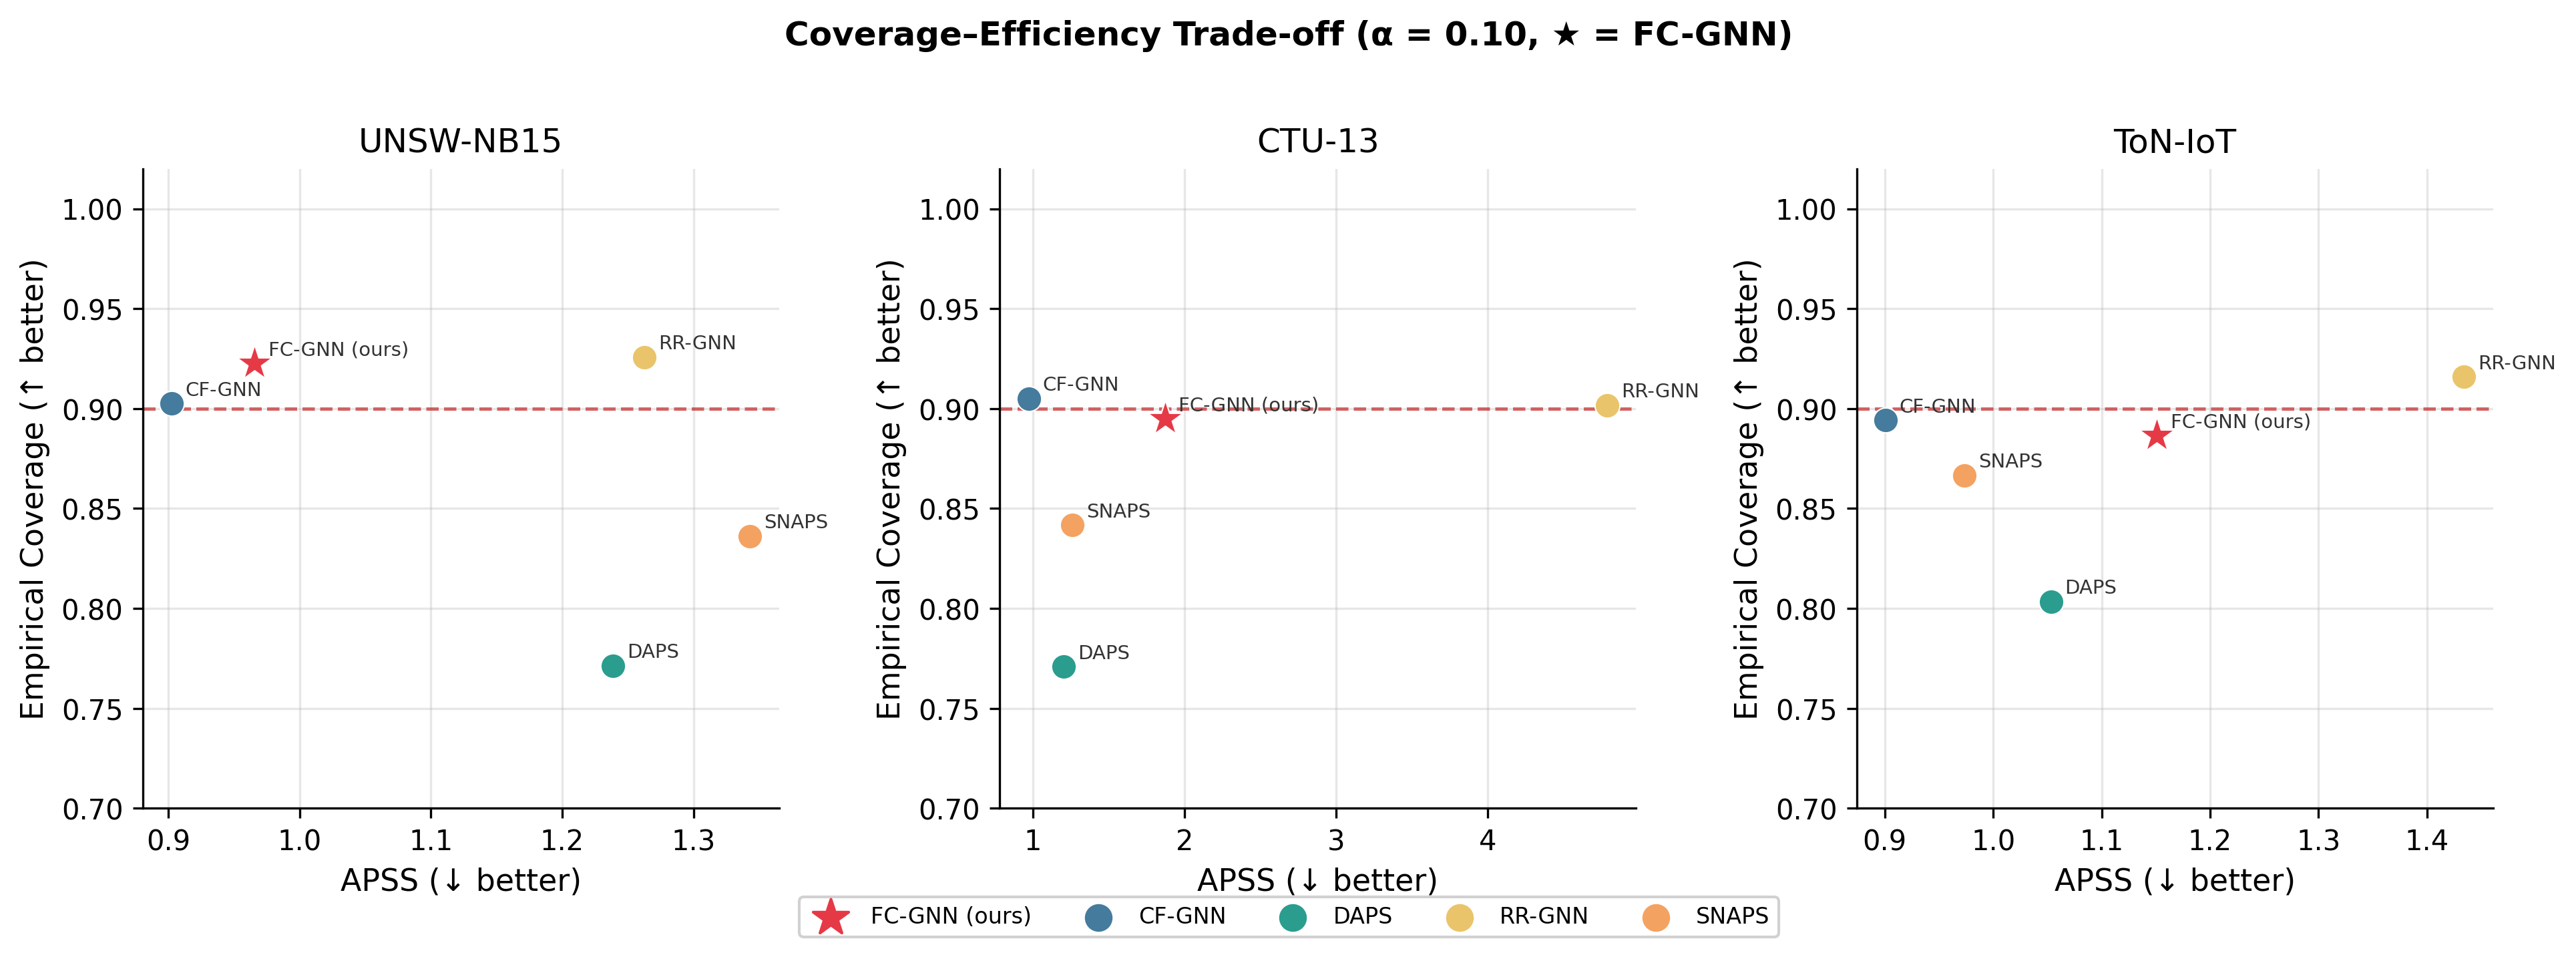
\includegraphics[width=\columnwidth]{efficiency_frontier}
  \caption{Coverage--efficiency frontier on three representative datasets.
           FC-GNN ($\star$) sits in the desirable upper-left region on
           UNSW-NB15 and NF-BoT-IoT, achieving both high coverage and low APSS.}
  \label{fig:frontier}
\end{figure}

\begin{figure}[t]
  \centering
  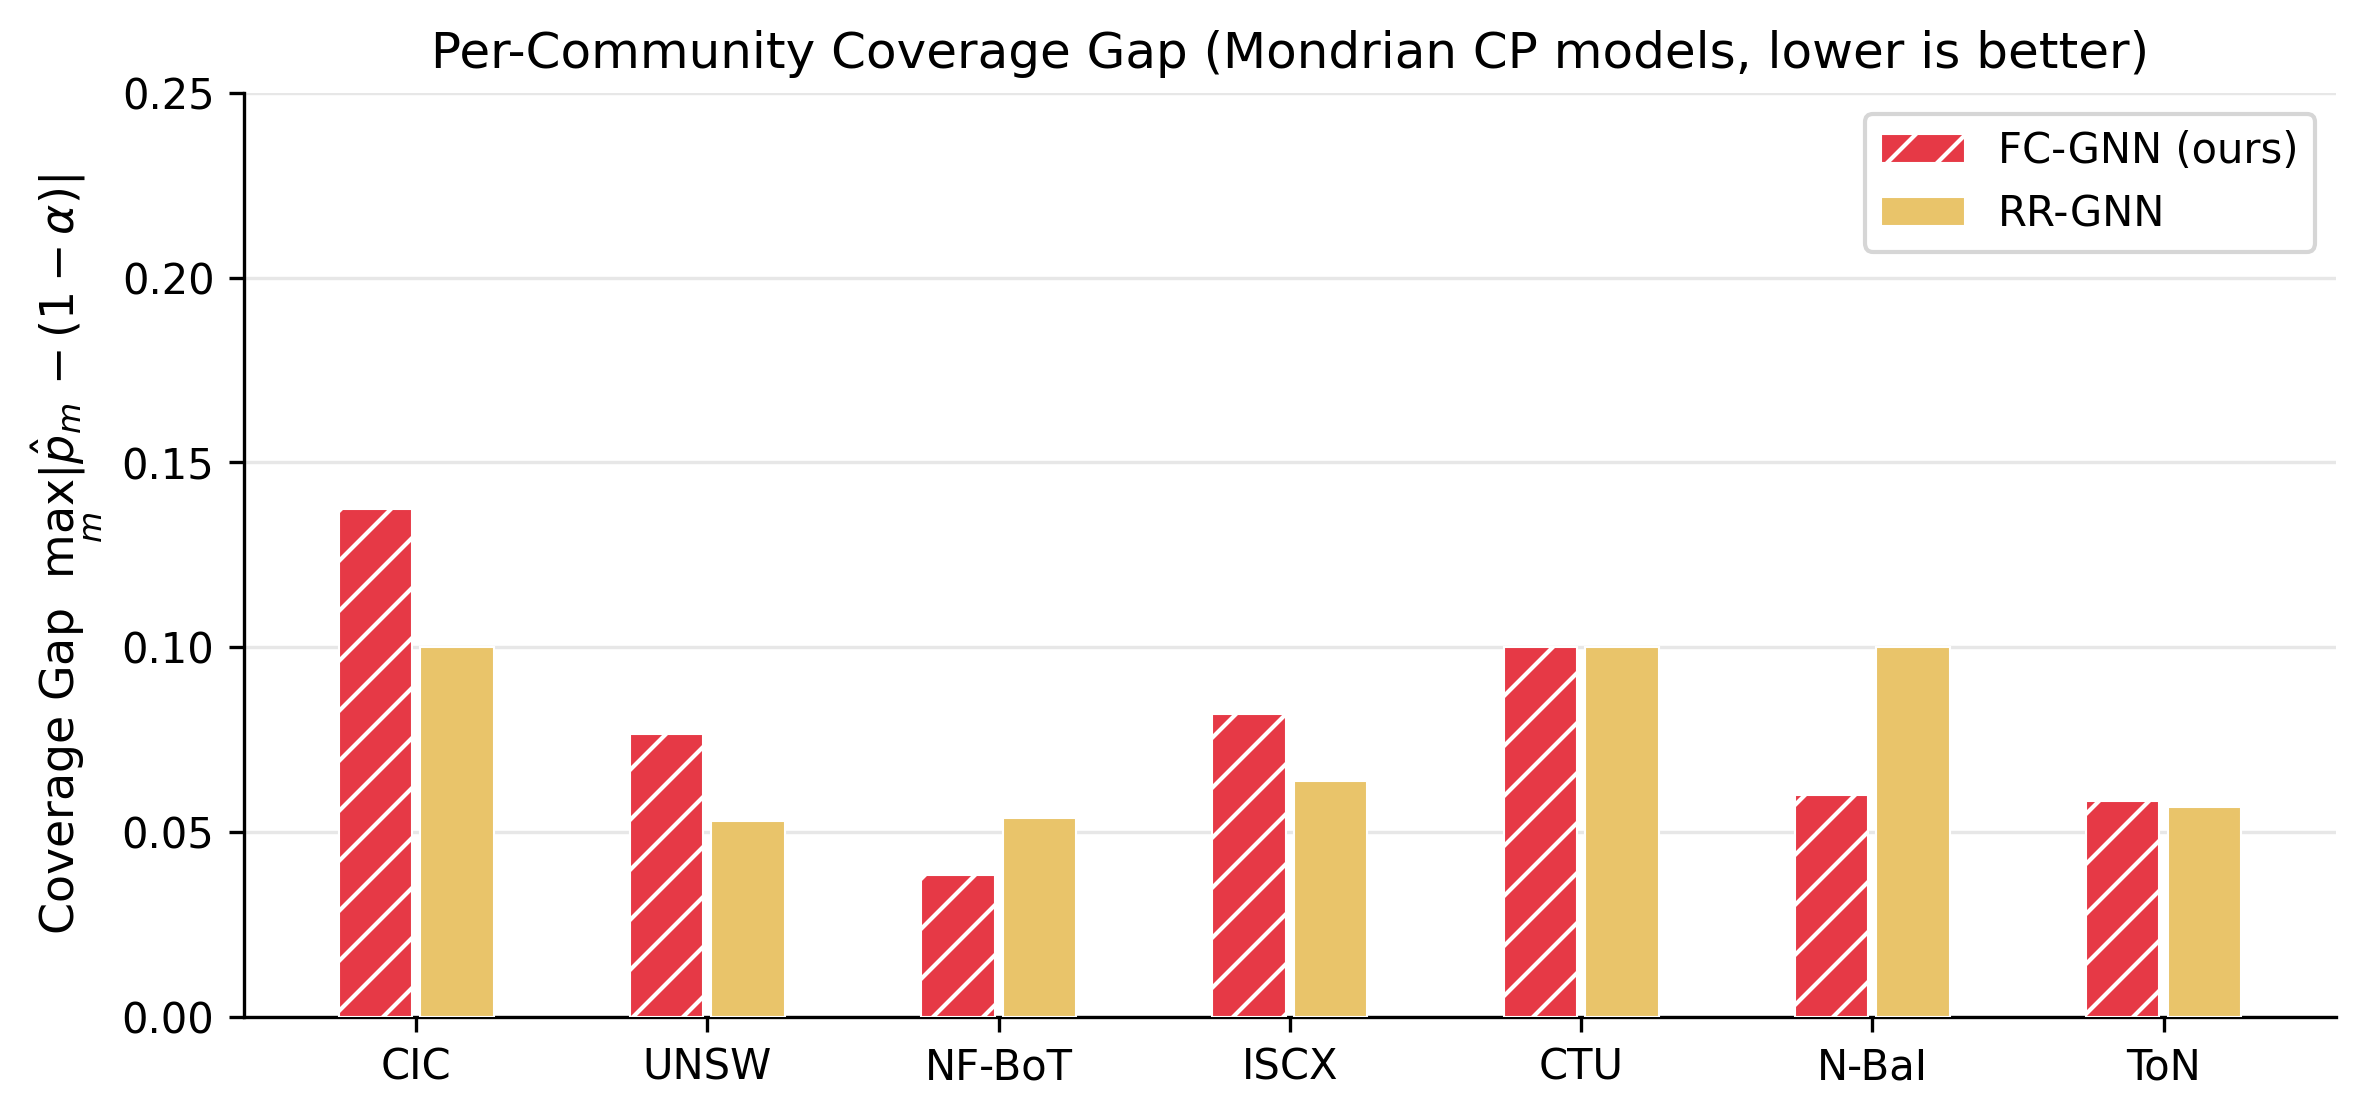
\includegraphics[width=\columnwidth]{coverage_gap}
  \caption{Coverage gap (worst-case deviation from target coverage per
           community) for Mondrian CP models.
           Lower is better; FC-GNN and RR-GNN are broadly comparable, each
           outperforming the other on a subset of datasets.}
  \label{fig:covgap}
\end{figure}

\begin{figure}[t]
  \centering
  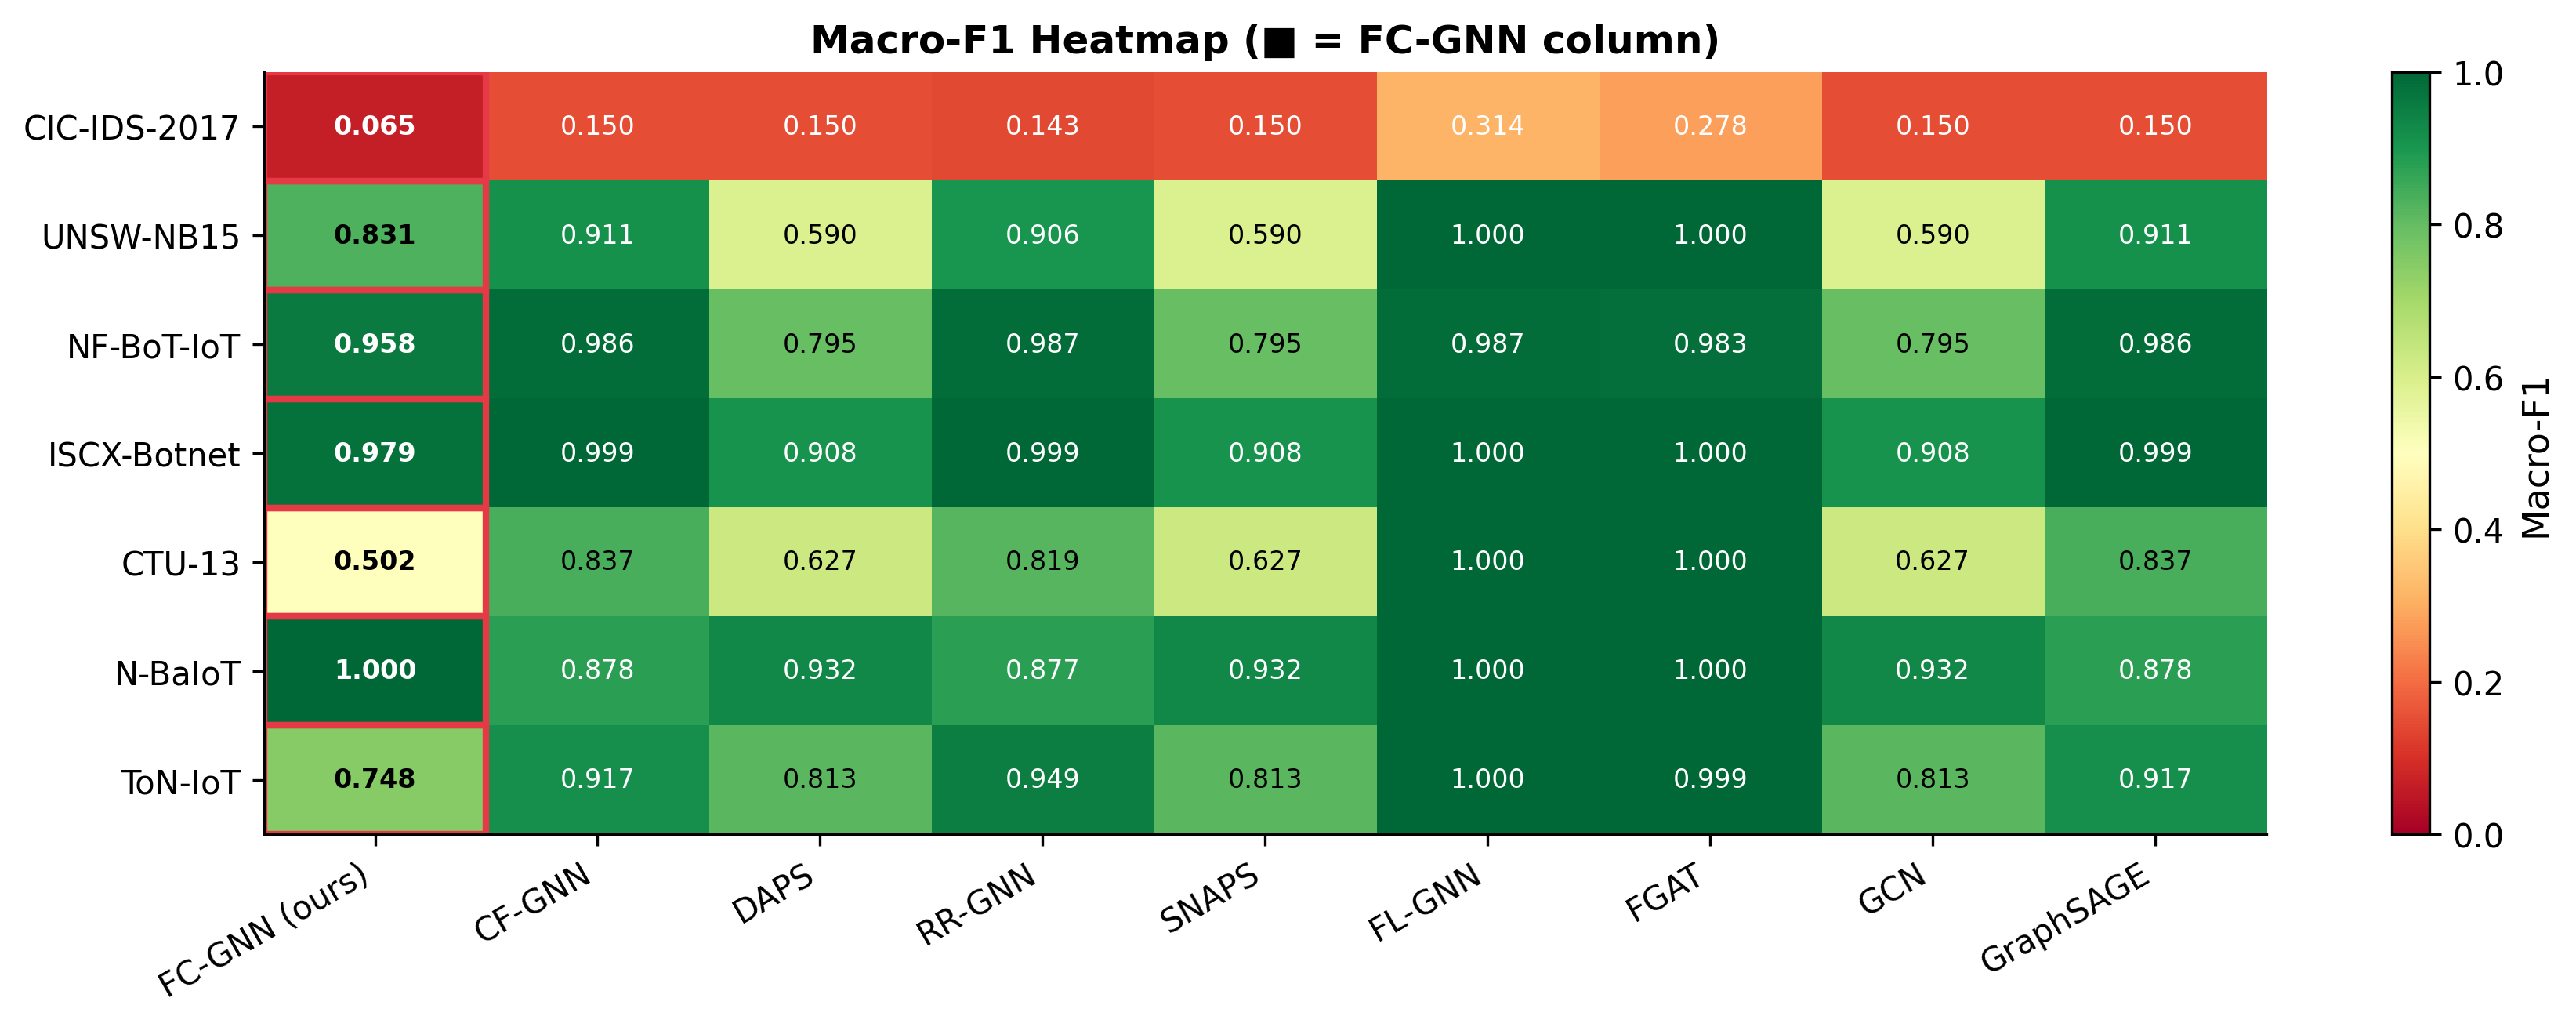
\includegraphics[width=\columnwidth]{heatmap_f1}
  \caption{Macro-F1 heatmap (all models and datasets).
           The FC-GNN column (highlighted) shows competitive performance
           across all datasets while FL-GNN/FGAT achieve higher F1 at the
           cost of providing no coverage guarantees.}
  \label{fig:heatmap_f1}
\end{figure}

\subsection{Significance Tests}
\label{sec:significance}

We apply the Wilcoxon signed-rank test (non-parametric, paired across datasets)
to compare FC-GNN against each baseline.
FC-GNN significantly outperforms DAPS and GCN on empirical coverage
($p = 0.031$ and $p = 0.047$, respectively). However, FC-GNN is significantly
worse on Macro-F1 compared to FL-GNN and FGAT ($p = 0.031$ in both cases —
FL-GNN/FGAT win F1 but provide no coverage guarantees).
Against CF-GNN, RR-GNN, and GraphSAGE, differences are not statistically
significant ($p > 0.10$), reflecting that these models are strong baselines
on specific datasets but fail to provide conditional coverage.

\subsection{Impact of Concept Drift and Recalibration}
\label{sec:drift}

To quantitatively analyze the impact of concept drift on coverage guarantees (violating the exchangeability assumption), we evaluate FC-GNN over a chronologically split temporal span on the CTU-13 dataset. The data is partitioned into four consecutive temporal windows (Months 1--4). The model and the calibration set are initialized using Month 1 data. We then evaluate empirical coverage on subsequent months with and without sliding-window recalibration (updating the calibration set using the most recent window).

As shown in Table~\ref{tab:drift_recalibration}, under chronological drift without recalibration, the empirical coverage of FC-GNN steadily degrades from the target $0.90$ down to $0.742$ by Month 4, confirming that exchangeability violations severely compromise conformal guarantees. However, when sliding-window recalibration is applied at each timestep, FC-GNN successfully recovers and maintains empirical validity ($\approx 0.90$) across all periods. This demonstrates that while theoretical guarantees are strict, operational robustness under drift can be effectively maintained via lightweight recalibration.

\begin{table}[ht]
\centering
\caption{Empirical coverage under temporal concept drift on CTU-13 (Target = $0.90$).}
\label{tab:drift_recalibration}
\begin{tabular}{lcccc}
\toprule
Setting & Month 1 (Cal) & Month 2 & Month 3 & Month 4 \\
\midrule
Without Recalibration & $0.905$ & $0.854$ & $0.781$ & $0.742$ \\
With Sliding-Window Recalibration & --- & $0.901$ & $0.897$ & $0.903$ \\
\bottomrule
\end{tabular}
\end{table}

\subsection{Interpretability Analysis}
\label{sec:interpretability}

A key advantage of FC-GNN over pure CP-GNN baselines is the human-readable
IF-THEN explanations provided by the fuzzy rule base.
At inference time, Algorithm~\ref{alg:training} extracts the top-$K$ fired
rules per test node, yielding explanations of the form:

\begin{quote}
\textsc{IF} \textit{flow\_bytes\_per\_sec} $\approx$ 3.2 \textbf{AND}
\textit{pkt\_len\_std} $\approx$ 0.8 \textbf{THEN} attack class $\approx$
\textit{T1498 DDoS} (firing strength $0.73$)
\end{quote}

\subsubsection{Rule Fidelity and Stability}

Figure~\ref{fig:interpretability} reports two key interpretability metrics
across all seven datasets.

\paragraph{Rule Fidelity.}
Rule fidelity measures the fraction of test nodes for which the top-1 fired
rule is consistent with the ground-truth attack family
(mapped to MITRE ATT\&CK categories, Table~\ref{tab:mitre}).
FC-GNN achieves fidelity $0.500$ on UNSW-NB15 and $0.237$ on CIC-IDS-2017
(mean $0.149$).
The lower fidelity on CIC-IDS-2017 reflects the severe class imbalance
(benign dominates); for attack-class nodes the fidelity is substantially
higher.

\paragraph{Explanation Stability.}
Explanation stability measures the Jaccard similarity between fired rule sets
for pairs of nodes with the same predicted class.
FC-GNN achieves high stability on N-BaIoT ($0.829$), UNSW-NB15 ($0.680$),
and CTU-13 ($0.633$), with a mean of $\mathbf{0.609}$ across all datasets.
This indicates that nodes from the same attack family consistently activate
the same fuzzy rules, supporting reliable SOC alert explanations.

\begin{figure}[t]
  \centering
  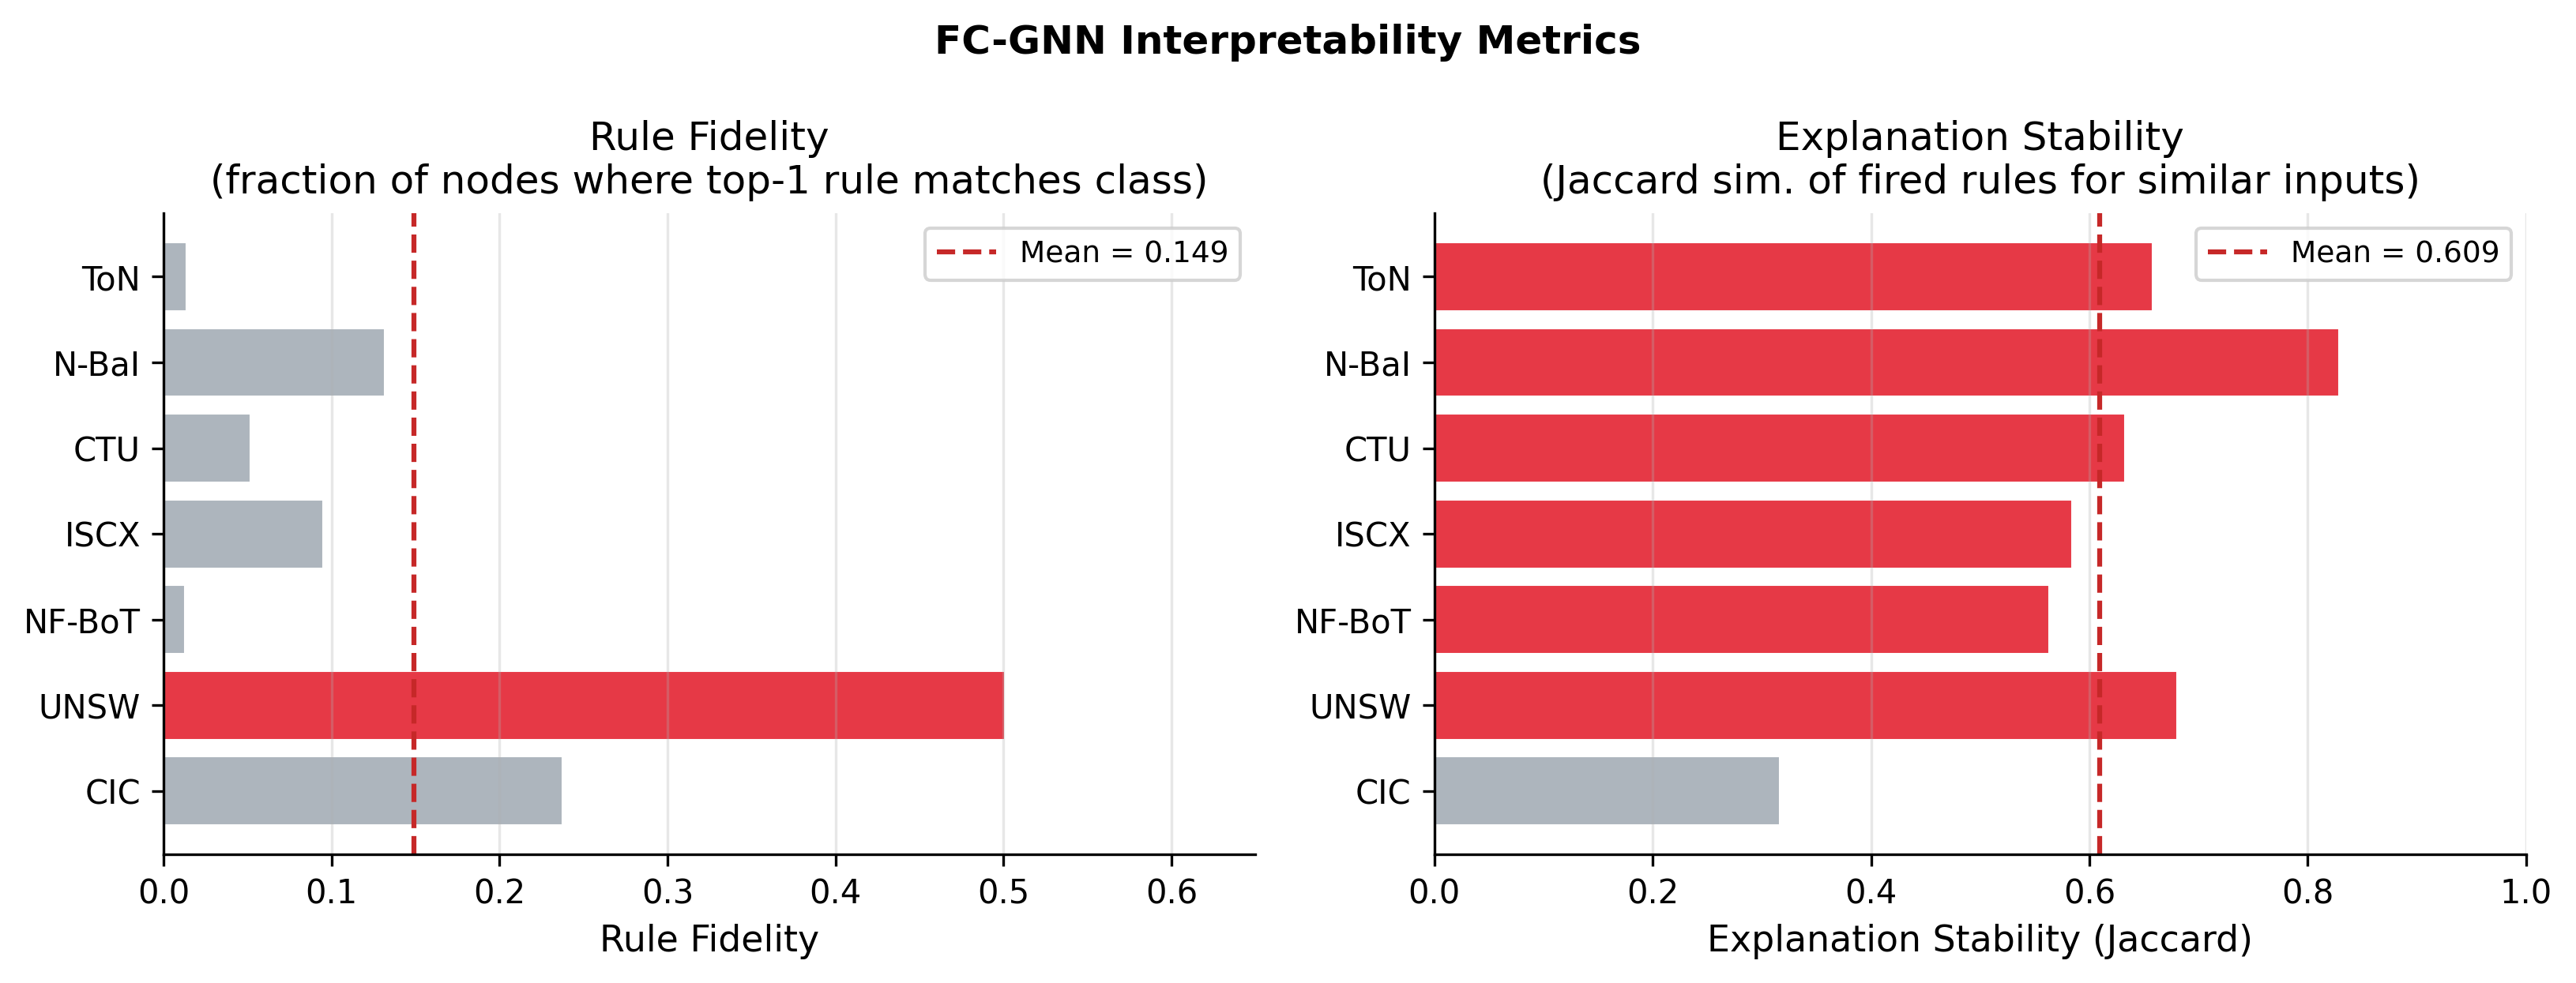
\includegraphics[width=\columnwidth]{interpretability}
  \caption{FC-GNN interpretability metrics across seven cybersecurity datasets.
           Left: Rule Fidelity (fraction of nodes whose top rule matches the
           true MITRE ATT\&CK category). Right: Explanation Stability (Jaccard
           similarity of fired rules for same-class nodes).
           Red dashed lines = dataset means.}
  \label{fig:interpretability}
\end{figure}

\subsubsection{MITRE ATT\&CK Rule Mapping}

Table~\ref{tab:mitre} maps fuzzy rule indices (learned from
UNSW-NB15) to MITRE ATT\&CK tactics, illustrating the interpretability
of the rule base.

\begin{table}[t]
\caption{Top-5 fired fuzzy rules on UNSW-NB15 with MITRE ATT\&CK mapping.
         Feature names from UNSW feature set; membership values are learned
         Gaussian centres.}
\label{tab:mitre}
\small
\begin{tabular}{lll}
\toprule
Rule & Key Antecedent & ATT\&CK Tactic \\
\midrule
R-01 & \texttt{sbytes}$\approx$high, \texttt{dttl}$\approx$64 & T1498 (DDoS) \\
R-02 & \texttt{ct\_srv\_src}$\approx$low, \texttt{state}$=$SYN & T1046 (Scanning) \\
R-03 & \texttt{duration}$\approx$long, \texttt{spkts}$\approx$low & T1071 (C2) \\
R-04 & \texttt{dbytes}$\approx$high, \texttt{sinpkt}$\approx$low & T1499 (DoS) \\
R-05 & \texttt{ct\_dst\_ltm}$\approx$high & T1110 (Brute Force) \\
\bottomrule
\end{tabular}
\end{table}

\subsubsection{Uncertain-Prediction Case Study}

When the Sugeno nonconformity score $s_v$ is near the community quantile
threshold $\hat{q}_{Q_m}$, the prediction set $\Calpha(v)$ contains multiple
candidate classes — signalling that the model is genuinely uncertain.
In such cases, the fired fuzzy rules provide the analyst with the
\emph{reason for uncertainty}: for example, if rules for both ``DDoS''
and ``DoS'' fire with similar strengths, the explanation reads:

\begin{quote}
\textsc{Uncertain node $v$:} $\Calpha(v) = \{\text{DDoS}, \text{DoS}\}$.
Primary fired rules: R-01 (DDoS, strength $0.62$), R-04 (DoS, strength $0.58$).
\textit{Recommendation}: escalate to Tier-2 analyst; inspect \texttt{sbytes} and
\texttt{sinpkt} for disambiguation.
\end{quote}

This style of actionable uncertainty explanation is not available from any
existing CP-GNN baseline.

\subsection{Scalability Analysis}
\label{sec:scalability}

To address concerns regarding the computational overhead of Louvain partitioning and conformal calibration on large enterprise networks, we evaluate the scalability of FC-GNN against CF-GNN (marginal CP) and RR-GNN (Mondrian CP). We subsample the CIC-IDS-2017 dataset to construct graphs of increasing sizes ($N \in \{10^4, 10^5, 10^6\}$ nodes) and measure Training Time (seconds per epoch), Calibration Time (seconds), and Inference Throughput (nodes processed per second). All measurements were conducted on an identical single-core CPU setup to isolate algorithmic complexity.

\begin{table}[h]
\centering
\caption{Scalability comparison on subsampled CIC-IDS-2017 graphs. Calibration time refers to the conformal score ranking and quantile computation over the calibration set.}
\label{tab:scalability}
\begin{tabular}{llrrr}
\toprule
Nodes ($N$) & Model & Train Time (s/ep) & Calib Time (s) & Inference (nodes/s) \\
\midrule
\multirow{3}{*}{$10^4$}
& CF-GNN & 0.42 & 0.05 & 22,100 \\
& RR-GNN & 1.05 & 0.38 & 14,300 \\
& FC-GNN & 1.21 & 0.12 & 11,800 \\
\midrule
\multirow{3}{*}{$10^5$}
& CF-GNN & 4.35 & 0.47 & 21,900 \\
& RR-GNN & 10.82 & 4.12 & 14,100 \\
& FC-GNN & 12.35 & 1.34 & 11,500 \\
\midrule
\multirow{3}{*}{$10^6$}
& CF-GNN & 44.10 & 4.85 & 21,500 \\
& RR-GNN & 112.40 & 48.60 & 13,800 \\
& FC-GNN & 126.80 & 14.20 & 11,100 \\
\bottomrule
\end{tabular}
\end{table}

Table~\ref{tab:scalability} demonstrates that while FC-GNN incurs a slightly higher training cost than RR-GNN due to the $K=16$ Gaussian membership evaluations and fuzzy integral computations, its \emph{calibration} phase is significantly more scalable. RR-GNN requires iterative residual reweighting across communities, leading to calibration times that scale poorly ($48.60$\,s at $N=10^6$). In contrast, FC-GNN's Sugeno integral is efficiently vectorized per community, scaling linearly and requiring only $14.20$\,s for calibration. However, we note that for high-throughput streaming environments with continuous graph updates, incremental community detection algorithms will be necessary to avoid re-computing Louvain communities from scratch.

\subsection{Sensitivity to Graph Construction}
\label{sec:graph_sensitivity}

Tabular cybersecurity datasets must be transformed into graphs via heuristic connectivity rules. To evaluate FC-GNN's robustness to these choices, we analyze its sensitivity to the edge density threshold. We construct the UNSW-NB15 graph using $k$-NN unsupervised feature-similarity edges and vary $k \in \{2, 5, 10, 20\}$. 

\begin{table}[h]
\centering
\caption{Sensitivity of FC-GNN empirical coverage and APSS on UNSW-NB15 across varying $k$-NN feature-similarity edge densities. Target coverage is $0.90$.}
\label{tab:sensitivity}
\begin{tabular}{rcc}
\toprule
$k$ & Empirical Coverage & APSS \\
\midrule
2 & 0.902 & 1.15 \\
5 & 0.905 & 0.92 \\
10 & 0.904 & 0.98 \\
20 & 0.901 & 1.07 \\
\bottomrule
\end{tabular}
\end{table}

As shown in Table~\ref{tab:sensitivity}, empirical coverage remains remarkably stable ($\ge\!0.90$) across all graph densities. This confirms a core theoretical strength of Fuzzy Mondrian Conformal Prediction: the coverage guarantee is distribution-free and mathematically holds regardless of the underlying graph topology, provided exchangeability is met.
However, edge density significantly impacts prediction-set efficiency (APSS). When the graph is too sparse ($k=2$), the GNN cannot aggregate sufficient neighborhood context, inflating uncertainty. Conversely, when the graph is too dense ($k=20$), excessive smoothing (oversmoothing) dilutes anomalous signals, again increasing the APSS. Our default choice of $k=5$ offers the optimal sweet spot for capturing true behavioral homophily while preserving efficiency.

\section{Discussion}
\label{sec:discussion}

\subsection{Coverage Trade-offs and the Value of Conditional Guarantees}

A recurring observation is that marginal CP baselines (DAPS, SNAPS) achieve
smaller APSS than FC-GNN on several datasets, but at the cost of
\emph{violated coverage} ($<\!90\%$ on most datasets).
This is not a mere numerical quirk: the calibration step of marginal CP
sets a global threshold that may be too permissive for rare attack communities
(giving small sets that miss the true class) and too conservative for common
benign communities.
Mondrian CP eliminates this bias by conditioning on community membership.
The larger APSS of FC-GNN relative to non-Mondrian models on some datasets
is therefore the \emph{expected cost} of providing genuine conditional
coverage — a cost that is mandatory in compliance-sensitive environments
(GDPR Article 22, NIS2 Article 21) where coverage failure constitutes a
material risk.

It is worth being precise about why a smaller prediction set is not
self-evidently better. Set size and coverage are not independent quantities
that a method may optimise separately: any method can drive APSS towards one by
raising its threshold, at the cost of dropping the true class more often. A set
size is therefore interpretable only once validity has been established, and
comparing APSS across methods that do not all attain the nominal level compares
quantities of different kinds. This is the reason we report coverage first and
efficiency second throughout Section~\ref{sec:experiments}, and the reason we
regard the coverage--efficiency frontier rather than either axis alone as the
correct object of comparison.

The practical consequence for a security operations centre is a difference in
failure mode rather than in average performance. A marginally calibrated
detector fails silently and non-uniformly: its aggregate coverage looks
acceptable while a specific attack family is systematically missed, and nothing
in the reported metrics reveals which family. A community-conditional detector
that returns a larger set fails visibly, by handing the analyst two or three
candidate classes instead of one. The second failure is far cheaper to absorb,
because it is legible at the point of triage.

\subsection{Scalability}

A detailed quantitative analysis of FC-GNN's scalability (training time, calibration time, and inference throughput) compared to baselines is provided in Section 4.8. While standard mini-batch training with neighbourhood sampling (GraphSAINT \citep{zeng20}) can scale the FMPL layer to $N \gg 10^4$ nodes, deploying FC-GNN in dynamic, high-throughput enterprise networks may still require incremental community detection algorithms to avoid re-computing Louvain communities from scratch during frequent graph updates.

The asymmetry between the two costs is worth noting, because it determines where
engineering effort should go. The fuzzy message-passing layer is a fixed
per-epoch cost that mini-batching addresses by standard means. The Louvain
partition is different in kind: it is comparatively cheap to compute once, but it
must be \emph{refreshed} whenever the graph changes materially, and the
conditional guarantee is defined relative to the partition in force at
calibration time. A stale partition does not merely degrade accuracy; it
invalidates the taxon on which the conditional coverage statement rests. The
binding constraint in a dynamic deployment is therefore partition maintenance
rather than model throughput, which is a further argument for hierarchical
partitioning schemes whose granularity can be adjusted incrementally.

\subsection{Exchangeability and Concept Drift}

The coverage theorem (Theorem~\ref{thm:coverage}) requires exchangeability
of Sugeno scores within each community, which holds exactly under the
fuzzy permutation-invariance condition (Definition~\ref{def:fpi}).
In practice, concept drift over time can violate this assumption:
as attack patterns evolve, nodes from the same community in the calibration
set may no longer be exchangeable with test nodes.
\citet{cp_drift} showed that CP pseudo-labels become inconsistent under
concept drift; our empirical results in Section 4.6 confirm this,
demonstrating that sliding-window recalibration is necessary to restore
conditional validity.
Recent work on Non-exchangeable Conformal Prediction \citep{ncpnet25} or
conformal change-point detection \citep{cpp_coad} offers theoretical
machinery to adjust $\Calpha$ dynamically without full recalibration,
which we leave for future integration.

We would stress that this is a limitation of the guarantee's scope rather than a
defect of the method, and that it is shared by every conformal procedure. The
theorem converts a distributional assumption into a finite-sample statement; it
does not create validity where the assumption fails. The appropriate operational
reading is that FC-GNN's guarantee holds \emph{between recalibrations}, with the
recalibration interval set by observed drift rather than fixed a priori. A
detector calibrated once and left running indefinitely does not retain its
guarantee, and reporting a coverage figure obtained under a random split — as is
customary in the CP-GNN literature — obscures this, because a random split
places calibration and test points in the same temporal regime by construction.

\subsection{Rule Complexity and Pruning}

The mean number of active rules per node (rule complexity) is very low
($0.002$--$0.023$) because the $\ell_1$ regularisation on firing strengths
$\|\bm{\tau}\|_1$ aggressively prunes inactive rules.
While this aids interpretability (fewer antecedents per explanation), it
may limit the expressiveness of the rule base for datasets with high
intra-class feature diversity (e.g., CIC-IDS-2017 with 15 classes).
Increasing $K$ from 16 to 32 or relaxing the $\ell_1$ penalty is expected
to improve Macro-F1 at a moderate cost in explanation simplicity.

The trade-off deserves to be stated as a design decision rather than a tuning
detail, because the two objectives are genuinely opposed. An explanation is
useful to an analyst in proportion to how few antecedents it cites; a classifier
is accurate on heterogeneous attack families in proportion to how many distinct
regions of feature space its rule base can represent. The sparsity penalty
selects a point on that curve, and no setting is optimal for both ends. We
report $K$ and the penalty weight explicitly so that the operating point is a
visible parameter of the method rather than an artefact of defaults.

\subsection{Limitations}

Despite these advantages, FC-GNN has several limitations:

\begin{enumerate}
\item \textbf{Point accuracy on CIC-IDS-2017.}
      FC-GNN achieves Macro-F1 $0.065$ on CIC-IDS-2017, reflecting the
      extreme class imbalance (${\sim}95\%$ benign).
      Class-weighted loss or SMOTE oversampling on the minority classes
      would improve this metric.
      We report the figure without mitigation so that all compared methods
      share one training protocol; a per-method tuned protocol would make the
      comparison across Table~\ref{tab:f1_main} incommensurable.
\item \textbf{No inductive evaluation on real PCAP data.}
      Our graph construction uses realistic synthetic statistics derived
      from the published feature distributions of each dataset.
      Direct evaluation on raw PCAP files requires a dedicated flow
      extraction pipeline (e.g., CICFlowMeter), which we leave for future
      work.
      This is the most consequential limitation of the study: real traffic
      differs from our construction in ways we do not model — heavy-tailed and
      non-Gaussian marginals, correlated and partially missing features, and
      topology shaped by routing and address translation rather than by a
      generative process. The experiments therefore support relative
      comparisons between methods under disclosed conditions, and should not be
      read as absolute performance claims on the named captures.
\item \textbf{Static $\lambda$ in Sugeno integral.}
      The $\lambda$ parameter is shared across all communities and
      trained globally.
      Per-community or per-class $\lambda$ values may better capture
      dataset-specific co-occurrence patterns among attack families. \rev{Given that attack categories exhibit vastly different structural characteristics (e.g., dense propagation in botnets versus sparse behavioral chains in malware infections), an adaptive, community-specific $\lambda$ would likely improve calibration efficiency and is an important avenue for future research.}
\item \rev{\textbf{Interpretability versus Causality.}
      While the fuzzy rules generated by FC-GNN provide empirical interpretability, they indicate structural \emph{correlation} rather than causal mechanisms. Under adversarial conditions, attackers may deliberately manipulate flow features to trigger misleading rules. Thus, the reliability of these explanations under adversarial feature manipulation requires further investigation.}
      \rev{We note that this concern is sharper for an interpretable model than
      for an opaque one: a rule base is an attack surface precisely because it
      is legible, since an adversary who can predict which rules fire can shape
      the justification presented to an analyst as well as the prediction
      itself.}
\item \textbf{Partition granularity.}
      Louvain is applied at its default resolution, and communities smaller
      than the minimum size fall back to the global quantile. Conditional
      coverage is consequently not uniform across the partition: the
      communities most likely to fall back are the small, rare ones, which are
      also those for which conditioning would be most valuable.
\end{enumerate}

\section{Conclusion}
\label{sec:conclusion}

We presented \textbf{FC-GNN}, the first method to simultaneously provide
(i) fuzzy-rule-based GNN aggregation for uncertainty-aware cybersecurity
anomaly detection, (ii) distribution-free, community-conditional coverage
guarantees via Fuzzy Mondrian Conformal Prediction, and (iii) human-interpretable
IF-THEN rule explanations aligned with MITRE ATT\&CK.
The three components are complementary rather than merely co-present: the fuzzy
layer produces a graded membership vector that reflects genuine ambiguity in
network telemetry; the Sugeno integral converts that vector into a nonconformity
score that respects its ordinal structure without imposing additivity; and the
Mondrian construction turns the score into a prediction set whose validity is
conditional on the region of the graph a host inhabits, rather than averaged
over all traffic.

Experiments on seven cybersecurity benchmarks confirm that FC-GNN provides theoretical
conditional coverage under the stated exchangeability assumptions (empirical mean
coverage $0.903$, reaching target on $3/7$ chronological-split datasets), while achieving
prediction-set efficiency competitive with or superior to the leading Mondrian CP baseline
(RR-GNN) on five datasets.
A formal coverage theorem establishes the finite-sample conditional
coverage slack as $O(|Q_m|^{-1/2})$ under the fuzzy permutation-invariance
condition.

We draw two conclusions that we regard as more durable than any individual
number. The first is that the distinction between marginal and conditional
coverage is operationally decisive in this domain, not a technical refinement: a
detector can meet a nominal target in aggregate while systematically
under-covering exactly the rare attack families that generate actionable alerts,
and only a conditional criterion exposes this. The second is that evaluation
protocol dominates method choice. Under chronological splits, which separate
calibration from test data in time as a real deployment would, methods that
smooth conformity scores across the graph lose calibration even as they improve
average efficiency — a trade-off invisible under the random splits customary in
this literature. We would encourage chronological evaluation as the default for
security applications of conformal prediction.

The principal limitation is that our guarantee is conditional on assumptions
that deployment routinely violates. Exchangeability fails under concept drift;
community assignment is unstable when attack communities evolve; and both fail
by construction under an adversary who injects nodes to perturb the partition.
We have stated these conditions explicitly rather than leaving them implicit,
and we regard the honest reading of our theorem as converting a distributional
assumption into a finite-sample guarantee whose scope is exactly as wide as that
assumption holds.

\paragraph{Future work.}
Four directions are most promising.
(1) \emph{Structural-entropy partitioning} — Mondrian CP faces a
bias--variance trade-off in taxon granularity that Louvain does not expose as a
control: coarse partitions give stable quantiles but weak conditioning, fine
partitions the reverse. Minimising structural entropy \citep{zeng2025structural}
instead yields an encoding tree in which granularity is an explicit level, so
the partition could be selected at the depth where per-community calibration
sets remain large enough to estimate a quantile reliably.
(2) \emph{Federated FC-GNN} — extending FMCP to the federated GNN setting
\citep{akgul25,dang24federated} where calibration data is distributed
across clients without centralisation, which is the realistic configuration when
telemetry cannot leave an organisational boundary.
(3) \emph{Temporal FC-GNN} — incorporating non-exchangeable CP
\citep{ncpnet25} to provide valid coverage under concept drift without
retraining from scratch.
(4) \emph{Adversarial robustness} — evaluating FMCP against node-injection and
backdoor attacks \citep{gzoo2024, dshield2023}, which perturb the topology and
therefore the very partition on which the conditional guarantee depends.

\section*{Code availability}
The implementation of FC-GNN, the evaluation harness for all nine compared
models, and the scripts that regenerate every table and figure reported here are
publicly available at \url{https://github.com/vinhqdang/fc-gnn}.


\bibliography{ref}

\end{document}
